% pdflatex -shell-escape foo.tex


\documentclass{article}
\usepackage{graphicx, amssymb, cite, amsmath, amsfonts, epsfig}
\usepackage{tikz} % Package for drawing
\usetikzlibrary{patterns}
\usetikzlibrary{spy}
\usepackage{pgfplots}
\usetikzlibrary{external}
\tikzexternalize[prefix=tikz/]



\newcommand{\floor}[1]{\lfloor #1 \rfloor}
\newcommand{\vecXA}{\vec{X}_A}
\newcommand{\vecXB}{\vec{X}_B}
\newcommand{\veca}{\vec{a}}


\DeclareMathOperator*{\ConvC}{\text{\raisebox{-0.45ex}{\scalebox{2.1}{$\boxtimes$}}}}
\DeclareMathOperator*{\ConvV}{\text{\raisebox{0.05ex}{\scalebox{2.1}{$\otimes$}}}}
\DeclareMathOperator*{\argmax}{argmax.}
\DeclareMathOperator*{\argmin}{argmin.}



\begin{document}



%--------------------------------------------------- Multidimentional recon

\begin{figure}[b]
  \begin{center}
    \resizebox{0.8\hsize}{!}{
      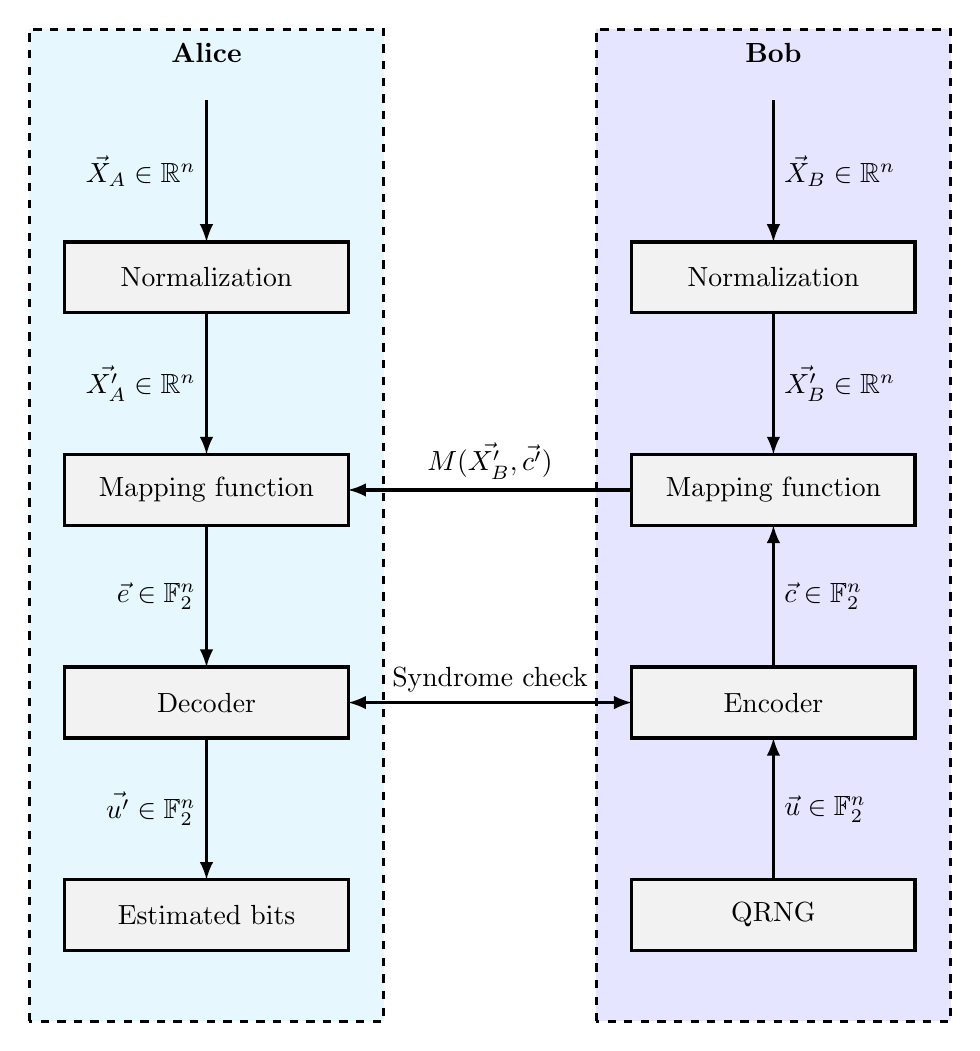
\begin{tikzpicture}[scale=0.90]
        %%-Alice
        \draw[black, very thick, dashed, fill=cyan!10!white] (-6.5,-6) rectangle ++(5,14) node[pos=0.5, yshift=6 cm] {\textbf{Alice}};
        
        \draw [black, very thick, >=latex] [->] (-4,7) -- (-4,5) node[left, pos=.5] { $\vecXA \in \mathbb{R}^n$};
        \draw[black, very thick, fill=gray!10!white] (-6,4) rectangle ++(4,1) node[pos=.5, yshift=.0 cm] {Normalization};
        \draw [black, very thick, >=latex] [->] (-4,4) -- (-4,2) node[left, pos=.5] { $\vec{X'_A} \in \mathbb{R}^n$};
        \draw[black, very thick, fill=gray!10!white] (-6,1) rectangle ++(4,1) node[pos=.5, yshift=.0 cm] {Mapping function};
        \draw [black, very thick, >=latex] [->] (-4,1) -- (-4,-1) node[left, pos=.5] { $\vec{e} \in \mathbb{F}_2^n$};
        \draw[black, very thick, fill=gray!10!white] (-6,-2) rectangle ++(4,1) node[pos=.5, yshift=.0 cm] {Decoder};
        \draw [black, very thick, >=latex] [->] (-4,-2) -- (-4,-4) node[left, pos=.5] { $\vec{u'} \in \mathbb{F}_2^n$};
         \draw[black, very thick, fill=gray!10!white] (-6,-5) rectangle ++(4,1) node[pos=.5, yshift=.0 cm] {Estimated bits};
        
        
         %% Bob
         \draw[black, very thick, dashed, fill=blue!10!white] (1.5,-6) rectangle ++(5,14) node[pos=0.5, yshift=6 cm] {\textbf{Bob}};
         
	\draw [black, very thick, >=latex] [->] (4,7) -- (4,5) node[right, pos=.5] { $\vecXB \in \mathbb{R}^n$};        
        \draw[black, very thick, fill=gray!10!white] (2,4) rectangle ++(4,1) node[pos=.5, yshift=.0 cm] {Normalization};
        \draw [black, very thick, >=latex] [->] (4,4) -- (4,2) node[right, pos=.5] { $\vec{X'_B} \in \mathbb{R}^n$};
        \draw[black, very thick, fill=gray!10!white] (2,1) rectangle ++(4,1) node[pos=.5, yshift=.0 cm] {Mapping function};
        \draw [black, very thick, >=latex] [<-] (4,1) -- (4,-1) node[right, pos=.5] { $\vec{c} \in \mathbb{F}_2^n$};
        \draw[black, very thick, fill=gray!10!white] (2,-2) rectangle ++(4,1) node[pos=.5, yshift=.0 cm] {Encoder};
        \draw [black, very thick, >=latex] [<-] (4,-2) -- (4,-4) node[right, pos=.5] { $\vec{u} \in \mathbb{F}_2^n$};
        \draw[black, very thick, fill=gray!10!white] (2,-5) rectangle ++(4,1) node[pos=.5, yshift=.0 cm] {QRNG};

%% classical channel
        \draw [black, very thick, >=latex] [->] (2,1.5) -- (-2,1.5) node[above, pos=.5] { $M(\vec{X'_B},\vec{c'})$};
        \draw [black, very thick, >=latex] [<->] (2,-1.5) -- (-2,-1.5) node[above, pos=.5] {Syndrome check};

        
        
      \end{tikzpicture}
    }
  \end{center}
  %\caption{Correlated source coding configuration. Correlated information sequences $\vecXB= (X_{B,0}, X_{B,1}, \ldots X_{B,n-1})$ and $\vecXA=(X_{A,0}, X_{A,1}, \ldots X_{A,n-1})$ are generated by a pair of continuous random variables $X_A, X_B$ from a given bivariate distribution $p_{X_AX_B}(x_A,x_B)$.}\label{fig:sourceCoding}
\end{figure}





\begin{figure}[b]
\begin{center}
\resizebox{0.8\hsize}{!}{
		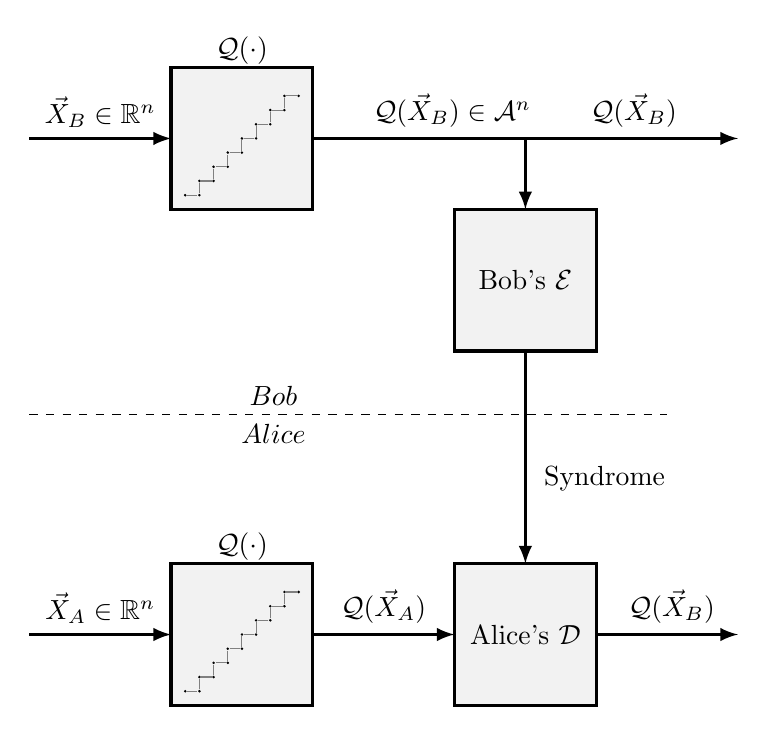
\begin{tikzpicture}[scale=0.90]
		\draw [black, very thick, >=latex] [->] (-4,2) -- (-2,2) node[above, pos=.5] { $\vecXB \in \mathbb{R}^n$};
		\draw[black, very thick, fill=gray!10!white] (-2,1) rectangle ++(2,2) node[above, pos=.5, yshift=.8 cm] {$\mathcal{Q}(\cdot)$};
%		
		\def\mypoints{(-1.8, 1.2),  (-1.6,1.2), (-1.6,1.4), (-1.4,1.4), (-1.4,1.6),
  (-1.2,1.6), (-1.2,1.8), (-1,1.8), (-1,2), (-.8,2), (-.8,2.2) , (-.6,2.2),   (-.6,2.4), (-.4,2.4), (-.4,2.6), (-.2,2.6)};
        \path
        \foreach \x [count=\xi] in \mypoints {
            \x node[circle, fill, inner sep=sqrt(2)*0.00025cm] (node\xi) {}
        }
        \foreach \x [count=\xi, remember=\xi-1 as \xiprev] in \mypoints {
            \ifnum\xi>1 %
            (node\xiprev) edge[>=latex, black!50!white] (node\xi)
            \fi
        };
		\draw [black, very thick, >=latex] [->] (0,2) -- (6,2) node[above, pos=.5] { $\mathcal{Q}(\vecXB) \in \mathcal{A}^n\,\,\,\,\,\,\,\quad \mathcal{Q}(\vecXB) $};
		\draw [black, very thick, >=latex] [->] (3,2) -- (3,1); % Vertical line
		\draw[black, very thick, fill=gray!10!white] (2,-1) rectangle ++(2,2) node[pos=.5] {Bob's $\mathcal{E}$};
		\draw [black, dashed, >=latex] [-] (-4,-1.9) -- (5,-1.9) node[below, xshift=-5 cm] { $Alice$} node[above, xshift=-5 cm] { $Bob$};
		\draw [black, very thick, >=latex] [->] (3,-1) -- (3,-4) node[right, xshift = .1 cm, pos = 0.6] {Syndrome}; % Vertical line
			\draw[black, very thick, fill=gray!10!white] (2,-6) rectangle ++(2,2) node[pos=.5] {Alice's $\mathcal{D}$};
		\draw [black, very thick, >=latex] [->] (-4,-5) -- (-2,-5) node[above, pos=.5] { $\vecXA \in \mathbb{R}^n$};
		\draw [black, very thick, >=latex] [->] (0,-5) -- (2,-5)node[above, pos=.5] { $\mathcal{Q}(\vecXA)$};
%		
		\draw[black, very thick, fill=gray!10!white] (-2,-6) rectangle ++(2,2) node[above, pos=.5, yshift=.8 cm] {$\mathcal{Q}(\cdot)$};
		\def\mypoints{(-1.8, -5.8),  (-1.6,-5.8), (-1.6,-5.6), (-1.4,-5.6), (-1.4,-5.4),
  (-1.2,-5.4), (-1.2,-5.2), (-1,-5.2), (-1,-5.0), (-.8,-5), (-.8,-4.8) , (-.6,-4.8),   (-.6,-4.6), (-.4,-4.6), (-.4,-4.4), (-.2,-4.4)};
        \path
        \foreach \x [count=\xi] in \mypoints {
            \x node[circle, fill, inner sep=sqrt(2)*0.00025cm] (node\xi) {}
        }
        \foreach \x [count=\xi, remember=\xi-1 as \xiprev] in \mypoints {
            \ifnum\xi>1 %
            (node\xiprev) edge[>=latex, black!50!white] (node\xi)
            \fi
        };
		\draw [black, very thick, >=latex] [->] (4,-5) -- (6,-5) node[above, pos=.5] { $\,\,\mathcal{Q}(\vecXB) $};
		\end{tikzpicture}
		}
	\end{center}
	%\caption{Correlated source coding configuration. Correlated information sequences $\vecXB= (X_{B,0}, X_{B,1}, \ldots X_{B,n-1})$ and $\vecXA=(X_{A,0}, X_{A,1}, \ldots X_{A,n-1})$ are generated by a pair of continuous random variables $X_A, X_B$ from a given bivariate distribution $p_{X_AX_B}(x_A,x_B)$.}\label{fig:sourceCoding}
\end{figure}




%% %----------------------------- source coding
%% \begin{figure}[!htbp]
%% \centering
%% \resizebox{0.70\textwidth}{!} {
%%   \begin{tikzpicture}[scale=0.75, dot/.style    = {anchor=base,fill,circle,inner sep=1.4pt}]    
%%     \draw [black, very thick, >=latex] [->] (-4,2) -- (-2,2) node[above, pos=.5] { $\vecXB \in \mathbb{R}^n$};
%%     \draw[black, very thick, fill=gray!10!white] (-2,1) rectangle ++(2,2) node[above, pos=.5, yshift=.8 cm] {$\mathcal{Q}(\cdot)$};
%%     %		
%%     \def\mypoints{(-1.8, 1.2),  (-1.6,1.2), (-1.6,1.4), (-1.4,1.4), (-1.4,1.6),
%%       (-1.2,1.6), (-1.2,1.8), (-1,1.8), (-1,2), (-.8,2), (-.8,2.2) , (-.6,2.2),   (-.6,2.4), (-.4,2.4), (-.4,2.6), (-.2,2.6)};
%%     \path
%%     \foreach \x [count=\xi] in \mypoints {
%%       \x node[circle, fill, inner sep=sqrt(2)*0.00025cm] (node\xi) {}
%%     }
%%     \foreach \x [count=\xi, remember=\xi-1 as \xiprev] in \mypoints {
%%       \ifnum\xi>1 %
%%       (node\xiprev) edge[>=latex, black!50!white] (node\xi)
%%       \fi
%%     };
%%     \draw [black, very thick, >=latex] [->] (0,2) -- (7,2) node[above, pos=.5] { $\mathcal{Q}(\vecXB) \in \mathcal{A}^n\,\,\,\,\,\,\,\quad \mathcal{Q}(\vecXB) $};
%%     \draw [black, very thick, >=latex] [->] (5,2) coordinate[dot] -- (5,1) node[right, xshift = .1 cm, pos = 0.5] {$X_B^3$}; % Vertical line
%%     \draw [black, very thick, >=latex] [->] (3,2) coordinate[dot] -- (3,-4)node[left, xshift = -.1 cm, pos = 0.1] {$X_B^2X_B^1X_B^0$}; % Vertical line
%%     \draw [black, very thick, >=latex] [->]  (3.25,2) coordinate[dot] -- (3.25,-4); % Vertical line
%%     \draw [black, very thick, >=latex] [->] (3.5,2) coordinate[dot] -- (3.5,-4); % Vertical line
%%     \draw [black, very thick, fill=gray!10!white] (4,-1) rectangle ++(2,2) node[pos=.5] {Bob's $\mathcal{E}$};
%%     \draw [black, dashed, >=latex] [-] (-4,-1.9) -- (7,-1.9) node[below, xshift=-7 cm] { $Alice$} node[above, xshift=-7 cm] { $Bob$};
%%     \draw [black, very thick, >=latex] [->] (5,-1) -- (5,-4) node[right, xshift = .1 cm, pos = 0.6] {$\vec{S}$}; % Vertical line
%%     \draw [black, very thick, fill=gray!10!white] (2,-6) rectangle ++(4,2) node[pos=.5] {Alice's $\mathcal{D}$};
%%     \draw [black, very thick, >=latex] [->] (-4,-5) -- (-2,-5) node[above, pos=.5] { $\vecXA \in \mathbb{R}^n$};
%%     \draw [black, very thick, >=latex] [->] (0,-5) -- (2,-5) node[above, pos=.5] { $\mathcal{Q}(\vecXA)$};
%%     \draw [black, very thick, >=latex] [->] (6,-5) -- (8,-5) node[above, pos=.5] { $\,\,\mathcal{Q}(\vecXB) $};
%%     %		
%%     \draw[black, very thick, fill=gray!10!white] (-2,-6) rectangle ++(2,2) node[above, pos=.5, yshift=.8 cm] {$\mathcal{Q}(\cdot)$};
    
%%     \def\mypoints{(-1.8, -5.8),  (-1.6,-5.8), (-1.6,-5.6), (-1.4,-5.6), (-1.4,-5.4),
%%       (-1.2,-5.4), (-1.2,-5.2), (-1,-5.2), (-1,-5.0), (-.8,-5), (-.8,-4.8) , (-.6,-4.8),   (-.6,-4.6), (-.4,-4.6), (-.4,-4.4), (-.2,-4.4)};
%%  \path
%%         \foreach \x [count=\xi] in \mypoints {
%%             \x node[circle, fill, inner sep=sqrt(2)*0.00025cm] (node\xi) {}
%%         }
%%         \foreach \x [count=\xi, remember=\xi-1 as \xiprev] in \mypoints {
%%             \ifnum\xi>1 %
%%             (node\xiprev) edge[>=latex, black!50!white] (node\xi)
%%             \fi
%%         };

    
%%     %% \path
%%     %% \foreach \x [count=\xi] in \mypointsss {
%%     %%   \x node[circle, fill, inner sep=sqrt(2)*0.00025cm] (node\xi) {}
%%     %% };
%%     %% \foreach \x [count=\xi, remember=\xi-1 as \xiprev] in \mypointsss {
%%     %%   \ifnum\xi>1 %
%%     %%   (node\xiprev) edge[>=latex, black!50!white] (node\xi)
%%     %%   \fi
%%     %% };
%%   \end{tikzpicture}
%% }
%% \end{figure}



%----------------------------- source coding one -level corrrect
\begin{figure}[!htbp]
\centering
\resizebox{0.70\textwidth}{!} {
  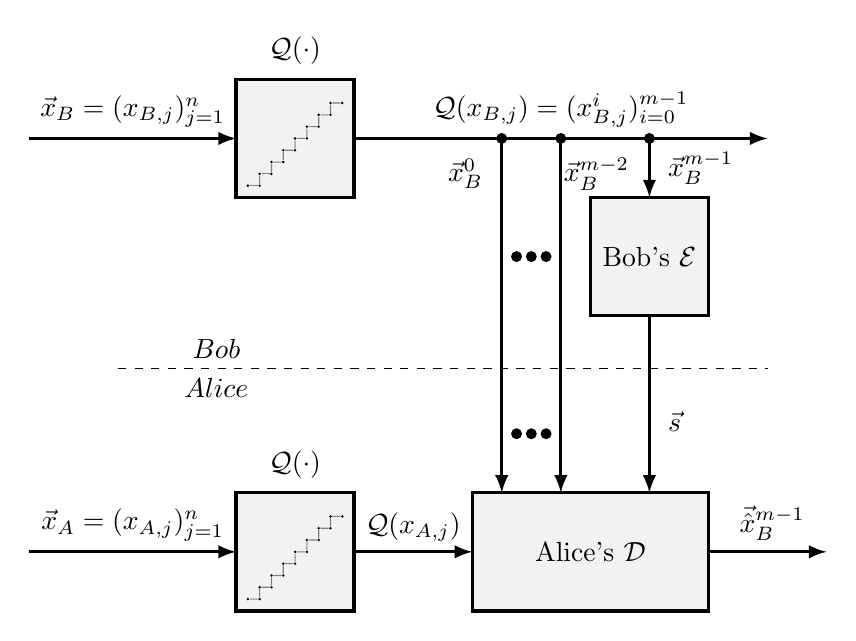
\begin{tikzpicture}[scale=0.75, dot/.style    = {anchor=base,fill,circle,inner sep=1.4pt}]    
    \draw [black, very thick, >=latex] [->] (-5.5,2) -- (-2,2) node[above, pos=.5] { $\vec{x}_B = (x_{B,j})_{j=1}^n$};
    \draw[black, very thick, fill=gray!10!white] (-2,1) rectangle ++(2,2) node[above, pos=.5, yshift=.8 cm] {$\mathcal{Q}(\cdot)$};
    %		
    \def\mypoints{(-1.8, 1.2),  (-1.6,1.2), (-1.6,1.4), (-1.4,1.4), (-1.4,1.6),
      (-1.2,1.6), (-1.2,1.8), (-1,1.8), (-1,2), (-.8,2), (-.8,2.2) , (-.6,2.2),   (-.6,2.4), (-.4,2.4), (-.4,2.6), (-.2,2.6)};
    \path
    \foreach \x [count=\xi] in \mypoints {
      \x node[circle, fill, inner sep=sqrt(2)*0.00025cm] (node\xi) {}
    }
    \foreach \x [count=\xi, remember=\xi-1 as \xiprev] in \mypoints {
      \ifnum\xi>1 %
      (node\xiprev) edge[>=latex, black!50!white] (node\xi)
      \fi
    };
    \draw [black, very thick, >=latex] [->] (0,2) -- (7,2) node[above, pos=.5] { $\mathcal{Q}(x_{B,j}) = (x_{B,j}^i)_{i=0}^{m-1}$};
    \draw [black, very thick, >=latex] [->] (5,2) coordinate[dot] -- (5,1) node[right, xshift = .1 cm, pos = 0.5] {$\vec{x}_B^{m-1}$}; % Vertical line
    \draw [black, very thick, >=latex] [->] (2.5,2) coordinate[dot] -- (2.5,-4)node[left, xshift = -.1 cm, pos = 0.1] {$\vec{x}_B^{0}$}; % Vertical line
    \draw (3.25,0) coordinate[dot]; % Vertical line
    \draw (3.00,0) coordinate[dot];
    \draw (2.75,0) coordinate[dot];
    \draw (3.25,-3) coordinate[dot]; % Vertical line
    \draw (3.00,-3) coordinate[dot];
    \draw (2.75,-3) coordinate[dot];
    \draw [black, very thick, >=latex] [->] (3.5,2) coordinate[dot] -- (3.5,-4) node[right, xshift = -0.1 cm, pos = 0.1] {$\vec{x}_B^{m-2}$};  % Vertical line
    \draw [black, very thick, fill=gray!10!white] (4,-1) rectangle ++(2,2) node[pos=.5] {Bob's $\mathcal{E}$};
    \draw [black, dashed, >=latex] [-] (-4,-1.9) -- (7,-1.9) node[below, xshift=-7 cm] { $Alice$} node[above, xshift=-7 cm] { $Bob$};
    \draw [black, very thick, >=latex] [->] (5,-1) -- (5,-4) node[right, xshift = .1 cm, pos = 0.6] {$\vec{s}$}; % Vertical line
    \draw [black, very thick, fill=gray!10!white] (2,-6) rectangle ++(4,2) node[pos=.5] {Alice's $\mathcal{D}$};
    \draw [black, very thick, >=latex] [->] (-5.5,-5) -- (-2,-5) node[above, pos=.5] { $\vec{x}_A = (x_{A,j})_{j=1}^n$};
    \draw [black, very thick, >=latex] [->] (0,-5) -- (2,-5) node[above, pos=.5] { $\mathcal{Q}(x_{A,j})$};
    \draw [black, very thick, >=latex] [->] (6,-5) -- (8,-5) node[above, pos=.5] { $\,\,\vec{\hat{x}}_B^{m-1} $};
    %		
    \draw[black, very thick, fill=gray!10!white] (-2,-6) rectangle ++(2,2) node[above, pos=.5, yshift=.8 cm] {$\mathcal{Q}(\cdot)$};
    
    \def\mypoints{(-1.8, -5.8),  (-1.6,-5.8), (-1.6,-5.6), (-1.4,-5.6), (-1.4,-5.4),
      (-1.2,-5.4), (-1.2,-5.2), (-1,-5.2), (-1,-5.0), (-.8,-5), (-.8,-4.8) , (-.6,-4.8),   (-.6,-4.6), (-.4,-4.6), (-.4,-4.4), (-.2,-4.4)};
 \path
        \foreach \x [count=\xi] in \mypoints {
            \x node[circle, fill, inner sep=sqrt(2)*0.00025cm] (node\xi) {}
        }
        \foreach \x [count=\xi, remember=\xi-1 as \xiprev] in \mypoints {
            \ifnum\xi>1 %
            (node\xiprev) edge[>=latex, black!50!white] (node\xi)
            \fi
        };
  \end{tikzpicture}
}
\end{figure}

%------------------------------- QUANTIZER

\begin{figure}[!ht]
  \centering
  \resizebox{0.85\textwidth}{!}{
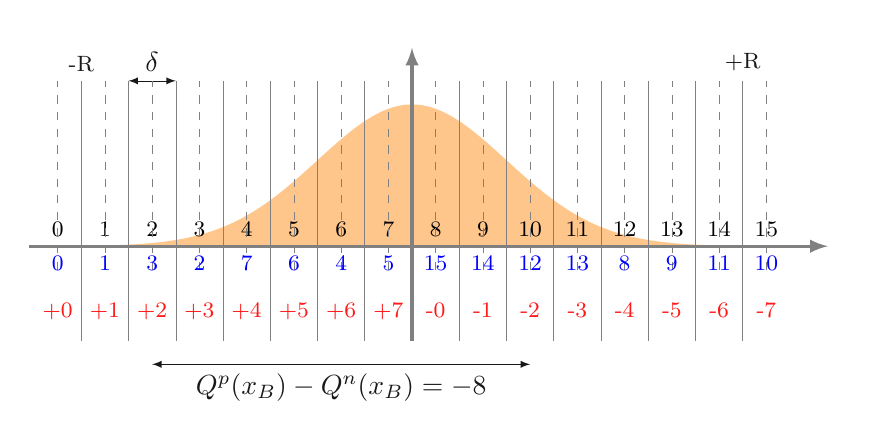
\begin{tikzpicture}[scale=.60, samples=100, >=latex]
    \def\Sig{2.0}
    % =========================
    %\draw[very thin, color= gray,  xshift = 0.0 cm] (-7.5,-3.5) grid (7.5,3.5);
    %\draw[very thin, color= gray, xshift = 0.5 cm] (-7.5,-3.5) grid (7.5,3.5);

    \fill[very thick, scale=1, domain=-7.5:7.5,smooth,variable=\x,orange!45] plot ({\x},{3*exp(-\x*\x/2/\Sig/\Sig)});
    \draw[very thick, ->, color= gray] (-8.1,0) -- (8.8,0) node[right] {};
    \draw[very thick, ->, color= gray] (0,-2.) -- (0,4.2) node[above] {};
    % ===============================
    \draw (-7,3.5) node[above, black!90]{\footnotesize{-R}};
    \draw (7,3.5) node[above, black!90]{\footnotesize{+R}};
    \draw[very thin, color= black!90, <->] (-6, 3.5) -- (-5,3.5) node[above, pos = 0.5]{$\delta$};
    \draw[very thin, color= black!90, <->] (-5.5, -2.5) -- (2.5,-2.5) node[below, pos = 0.5]{$Q^p(x_B)-Q^n(x_B) = -8$};
    
    \foreach \x in {-7.5,...,7.5}
        {\pgfmathtruncatemacro{\label}{\x +7.5}
        \draw (\x,0) node[above]{\footnotesize{{\label}}};}
        
    \foreach \x in {-7.5,...,7.5}    
        \draw[very thin, color= gray, dashed] (\x, -.5) -- (\x,3.5) ;
    
    \foreach \x in {-7.0,...,7.0}    
        \draw[very thin, color= gray] (\x, -2.) -- (\x,3.5) ;
    
    % \foreach \x in {-7.5,...,-0.5}
    %     {\pgfmathtruncatemacro{\label}{\x +7.5}
    %     \draw (\x,0) node[below]{\footnotesize{{\label}}};}    
%\draw[very thin, color= blue!60, -, dashed] (-8, -1.) -- (8.,-1.);  
%\draw[very thin, color= blue!60, -, dashed] (-8, -2.) -- (8.,-2.);
   \def\mypoints{0, 1, 3, 2, 7, 6, 4, 5, 15, 14, 12, 13, 8, 9, 11, 10};
   \foreach \x [count=\xi] in \mypoints {
            \draw (\xi-8.5,0) node[blue, below]{\footnotesize{\x}};
        } 
    \foreach \x [count=\xi] in {0, ..., 7} {
        \draw (\xi-8.5,-1) node[red!90, below]{\footnotesize{+\x}};
        \draw (\xi-.5,-1) node[red!90, below]{\footnotesize{-\x}};
        }
 %\draw[very thin, color= red!60, -, dashed] (-8., -4.) -- (8.,-4.); 
\end{tikzpicture}
}
%% \caption{A quantizer with $4$ bits. It provides $16$ non-overlapping intervals. The binary, Grey and sign-magnitude mappings are also considered. It is clear that, the distance between two points with equal LSBs is always fixed and it is equal to $8$}\label{fig:quantizer}
\end{figure}







%----------------------------- reconciliation two levels New          
\begin{figure}[!ht]
\centering
\resizebox{0.7\hsize}{!}{
		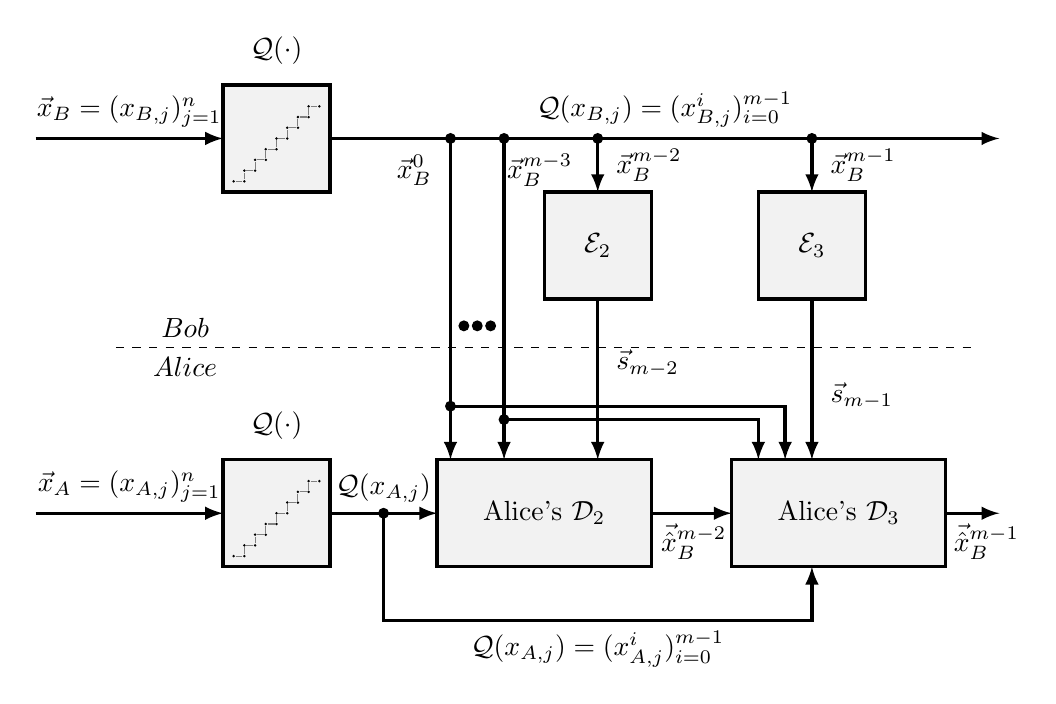
\begin{tikzpicture}[scale=0.68, dot/.style    = {anchor=base,fill,circle,inner sep=1.4pt}]
		
		\draw [black, very thick, >=latex] [->] (-5.5,2) -- (-2,2) node[above, pos=.5] {$\vec{x}_B = (x_{B,j})_{j=1}^n$};
		\draw[black, very thick, fill=gray!10!white] (-2,1) rectangle ++(2,2) node[above, pos=.5, yshift=.8 cm] {$\mathcal{Q}(\cdot)$};
%		
		\def\mypoints{(-1.8, 1.2),  (-1.6,1.2), (-1.6,1.4), (-1.4,1.4), (-1.4,1.6),
  (-1.2,1.6), (-1.2,1.8), (-1,1.8), (-1,2), (-.8,2), (-.8,2.2) , (-.6,2.2),   (-.6,2.4), (-.4,2.4), (-.4,2.6), (-.2,2.6)};
        \path
        \foreach \x [count=\xi] in \mypoints {
            \x node[circle, fill, inner sep=sqrt(2)*0.00025cm] (node\xi) {}
        }
        \foreach \x [count=\xi, remember=\xi-1 as \xiprev] in \mypoints {
            \ifnum\xi>1 %
            (node\xiprev) edge[>=latex, black!50!white] (node\xi)
            \fi
        };
		\draw [black, very thick, >=latex] [->] (0,2) -- (12.5,2) node[above, pos=.5] {$\mathcal{Q}(x_{B,j}) = (x_{B,j}^i)_{i=0}^{m-1}$};
		\draw [black, very thick, >=latex] [->] (5,2) coordinate[dot] -- (5,1) node[right, xshift = .1 cm, pos = 0.5] {$\vec{x}_B^{m-2}$}; % Vertical line
		%\draw [black, very thick, >=latex] [->] (3,2) coordinate[dot] -- (3,-4); % Vertical line
		\draw [black, very thick, >=latex] [->]  (3.25,2) coordinate[dot] -- (3.25,-4)node[right, xshift = -.1 cm, pos = 0.1, rotate = 00] {$\vec{x}_B^{m-3}$}; % Vertical line
                \draw [black, very thick, >=latex] [->]  (2.25,2) coordinate[dot] -- (2.25,-4)node[left, xshift = -.1 cm, pos = 0.1, rotate = 00] {$\vec{x}_B^{0}$}; % Vertical line
                \draw (2.50,-1.5) coordinate[dot]; % Vertical line
                \draw (2.75,-1.5) coordinate[dot]; % Vertical line
                \draw (3.00,-1.5) coordinate[dot]; % Vertical line
		\draw [black, very thick, >=latex] [->] (9,2) coordinate[dot] -- (9,1) node[right, xshift = .1 cm, pos = 0.5] {$\vec{x}_B^{m-1}$}; % Vertical line
		\draw[black, very thick, fill=gray!10!white] (4,-1) rectangle ++(2,2) node[pos=.5] {$\mathcal{E}_2$};
		\draw[black, very thick, fill=gray!10!white] (8,-1) rectangle ++(2,2) node[pos=.5] {$\mathcal{E}_3$};
		\draw [black, dashed, >=latex] [-] (-4,-1.9) -- (12,-1.9) node[below, xshift=-10 cm] { $Alice$} node[above, xshift=-10 cm] { $Bob$};
		%%%%%%%%%%%%%%%%%%% Level 2
		\draw [black, very thick, >=latex] [->] (5,-1) -- (5,-4) node[right, xshift = .1 cm, pos = 0.4] {$\vec{s}_{m-2}$}; % Vertical line
			\draw[black, very thick, fill=gray!10!white] (2,-6) rectangle ++(4,2) node[pos=.5] {Alice's $\mathcal{D}_2$};
	    \draw [black, very thick, >=latex] [->] (6,-5) -- (7.5,-5) node[below, pos=.5] { $\,\vec{\hat{x}}_B^{m-2} $};
        %%%%%%%%%%%%%%%%%%% Level 3
		\draw [black, very thick, >=latex] [->] (9,-1) -- (9,-4) node[right, xshift = .1 cm, pos = 0.6] {$\vec{s}_{m-1}$}; % Vertical line
			\draw[black, very thick, fill=gray!10!white] (7.5,-6) rectangle ++(4,2) node[pos=.5] {Alice's $\mathcal{D}_3$};
        \draw [black, very thick, >=latex] [->] (11.5,-5) -- (12.5,-5) node[below, pos=.5] { $\,\,~~\vec{\hat{x}}_B^{m-1}$};			
		\draw [black, very thick, >=latex] [->] (-5.5,-5) -- (-2,-5) node[above, pos=.5] {$\vec{x}_A = (x_{A,j})_{j=1}^n$};
		\draw [black, very thick, >=latex] [->] (0,-5) -- (2,-5) node[above, pos=.5] { $\mathcal{Q}(x_{A,j})$};
		\draw [black, very thick, >=latex] [->] (1,-5) coordinate[dot] -- (1,-7) -- (9,-7)node[below, pos=.5] { $\mathcal{Q}(x_{A,j}) = (x_{A,j}^i)_{i=0}^{m-1}$} -- (9, -6);
		\draw [black, very thick, >=latex] [->] (2.25,-3) coordinate[dot] -- (8.5,-3) -- (8.5,-4);
		\draw [black, very thick, >=latex] [->] (3.25,-3.25) coordinate[dot] -- (8.0,-3.25) -- (8.0,-4);
%		
		\draw[black, very thick, fill=gray!10!white] (-2,-6) rectangle ++(2,2) node[above, pos=.5, yshift=.8 cm] {$\mathcal{Q}(\cdot)$};
		\def\mypoints{(-1.8, -5.8),  (-1.6,-5.8), (-1.6,-5.6), (-1.4,-5.6), (-1.4,-5.4),
  (-1.2,-5.4), (-1.2,-5.2), (-1,-5.2), (-1,-5.0), (-.8,-5), (-.8,-4.8) , (-.6,-4.8),   (-.6,-4.6), (-.4,-4.6), (-.4,-4.4), (-.2,-4.4)};
        \path
        \foreach \x [count=\xi] in \mypoints {
            \x node[circle, fill, inner sep=sqrt(2)*0.00025cm] (node\xi) {}
        }
        \foreach \x [count=\xi, remember=\xi-1 as \xiprev] in \mypoints {
            \ifnum\xi>1 %
            (node\xiprev) edge[>=latex, black!50!white] (node\xi)
            \fi
        };
		
		\end{tikzpicture}
		}
	%% \caption{The reverse reconciliation, when two most significant bits are encoded}\label{fig:sourceCoding_twolevels}
\end{figure}














%----------------------------- reconciliation two levels
%% \begin{figure}[!ht]
%% \centering
%% \resizebox{0.7\hsize}{!}{
%% 		\begin{tikzpicture}[scale=0.68, dot/.style    = {anchor=base,fill,circle,inner sep=1.4pt}]
		
%% 		\draw [black, very thick, >=latex] [->] (-4,2) -- (-2,2) node[above, pos=.5] { $\vecXB \in \mathbb{R}^n$};
%% 		\draw[black, very thick, fill=gray!10!white] (-2,1) rectangle ++(2,2) node[above, pos=.5, yshift=.8 cm] {$\mathcal{Q}(\cdot)$};
%% %		
%% 		\def\mypoints{(-1.8, 1.2),  (-1.6,1.2), (-1.6,1.4), (-1.4,1.4), (-1.4,1.6),
%%   (-1.2,1.6), (-1.2,1.8), (-1,1.8), (-1,2), (-.8,2), (-.8,2.2) , (-.6,2.2),   (-.6,2.4), (-.4,2.4), (-.4,2.6), (-.2,2.6)};
%%         \path
%%         \foreach \x [count=\xi] in \mypoints {
%%             \x node[circle, fill, inner sep=sqrt(2)*0.00025cm] (node\xi) {}
%%         }
%%         \foreach \x [count=\xi, remember=\xi-1 as \xiprev] in \mypoints {
%%             \ifnum\xi>1 %
%%             (node\xiprev) edge[>=latex, black!50!white] (node\xi)
%%             \fi
%%         };
%% 		\draw [black, very thick, >=latex] [->] (0,2) -- (12,2) node[above, pos=.5] { $\mathcal{Q}(\vecXB) \in \mathcal{A}^n$};
%% 		\draw [black, very thick, >=latex] [->] (5,2) coordinate[dot] -- (5,1) node[right, xshift = .1 cm, pos = 0.5] {$X_B^2$}; % Vertical line
%% 		\draw [black, very thick, >=latex] [->] (3,2) coordinate[dot] -- (3,-4)node[left, xshift = -.1 cm, pos = 0.1] {$X_B^1X_B^0$}; % Vertical line
%% 		\draw [black, very thick, >=latex] [->]  (3.25,2) coordinate[dot] -- (3.25,-4); % Vertical line
%% 		\draw [black, very thick, >=latex] [->] (9,2) coordinate[dot] -- (9,1) node[right, xshift = .1 cm, pos = 0.5] {$X_B^3$}; % Vertical line
%% 		\draw[black, very thick, fill=gray!10!white] (4,-1) rectangle ++(2,2) node[pos=.5] {$\mathcal{E}_2$};
%% 		\draw[black, very thick, fill=gray!10!white] (8,-1) rectangle ++(2,2) node[pos=.5] {$\mathcal{E}_3$};
%% 		\draw [black, dashed, >=latex] [-] (-4,-1.9) -- (12,-1.9) node[below, xshift=-10 cm] { $Alice$} node[above, xshift=-10 cm] { $Bob$};
%% 		%%%%%%%%%%%%%%%%%%% Level 2
%% 		\draw [black, very thick, >=latex] [->] (5,-1) -- (5,-4) node[right, xshift = .1 cm, pos = 0.4] {$\vec{S}_2$}; % Vertical line
%% 			\draw[black, very thick, fill=gray!10!white] (2,-6) rectangle ++(4,2) node[pos=.5] {Alice's $\mathcal{D}_2$};
%% 	    \draw [black, very thick, >=latex] [->] (6,-5) -- (7,-5) node[below, pos=.5] { $\,\,X_B^2 $};
%%         %%%%%%%%%%%%%%%%%%% Level 3
%% 		\draw [black, very thick, >=latex] [->] (9,-1) -- (9,-4) node[right, xshift = .1 cm, pos = 0.6] {$\vec{S}_3$}; % Vertical line
%% 			\draw[black, very thick, fill=gray!10!white] (7,-6) rectangle ++(4,2) node[pos=.5] {Alice's $\mathcal{D}_3$};
%%         \draw [black, very thick, >=latex] [->] (11,-5) -- (12,-5) node[below, pos=.5] { $\,\,X_B^3 $};			
%% 		\draw [black, very thick, >=latex] [->] (-4,-5) -- (-2,-5) node[above, pos=.5] { $\vecXA \in \mathbb{R}^n$};
%% 		\draw [black, very thick, >=latex] [->] (0,-5) -- (2,-5) node[above, pos=.5] { $\mathcal{Q}(\vecXA)$};
%% 		\draw [black, very thick, >=latex] [->] (1,-5) coordinate[dot] -- (1,-7) -- (9,-7) -- (9, -6);
%% 		\draw [black, very thick, >=latex] [->] (3,-3) coordinate[dot] -- (8.25,-3) -- (8.25,-4);
%% 		\draw [black, very thick, >=latex] [->] (3.25,-3.25) coordinate[dot] -- (7.5,-3.25) -- (7.5,-4);
%% %		
%% 		\draw[black, very thick, fill=gray!10!white] (-2,-6) rectangle ++(2,2) node[above, pos=.5, yshift=.8 cm] {$\mathcal{Q}(\cdot)$};
%% 		\def\mypoints{(-1.8, -5.8),  (-1.6,-5.8), (-1.6,-5.6), (-1.4,-5.6), (-1.4,-5.4),
%%   (-1.2,-5.4), (-1.2,-5.2), (-1,-5.2), (-1,-5.0), (-.8,-5), (-.8,-4.8) , (-.6,-4.8),   (-.6,-4.6), (-.4,-4.6), (-.4,-4.4), (-.2,-4.4)};
%%         \path
%%         \foreach \x [count=\xi] in \mypoints {
%%             \x node[circle, fill, inner sep=sqrt(2)*0.00025cm] (node\xi) {}
%%         }
%%         \foreach \x [count=\xi, remember=\xi-1 as \xiprev] in \mypoints {
%%             \ifnum\xi>1 %
%%             (node\xiprev) edge[>=latex, black!50!white] (node\xi)
%%             \fi
%%         };
		
%% 		\end{tikzpicture}
%% 		}
%% 	%% \caption{The reverse reconciliation, when two most significant bits are encoded}\label{fig:sourceCoding_twolevels}
%% \end{figure}


%------------------------------- MLC-MSD reverse
\begin{figure*}[!ht]
	\centering
% 		{%\resizebox{14cm}{9 cm}
		\resizebox{0.7\textwidth}{!}{
			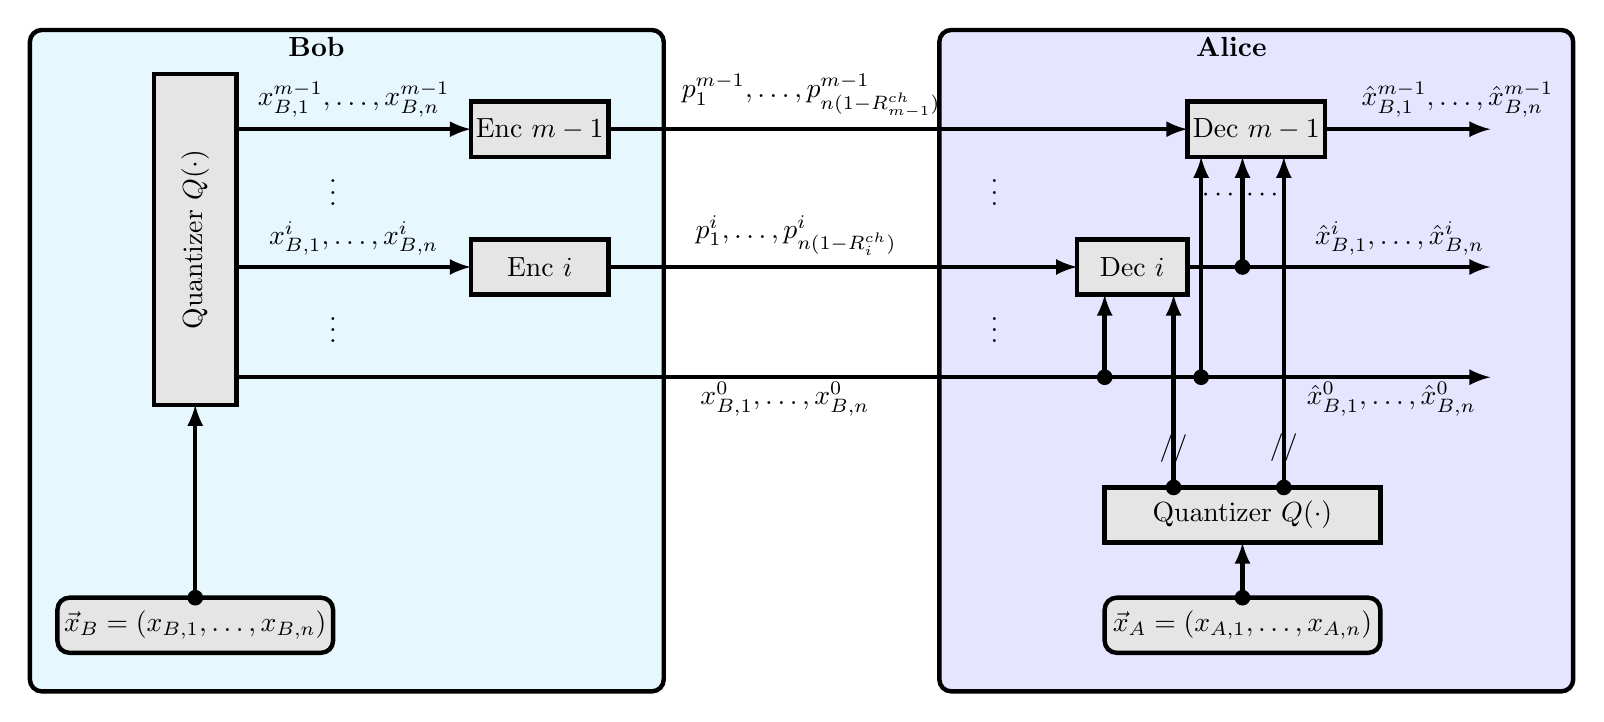
\begin{tikzpicture}[scale=0.7, 
			dot/.style    = {anchor=base,fill,circle,inner sep=2pt},
			block_1/.style  = {draw, rectangle, black, ultra thick, fill=gray!30!white, minimum width = 0.75cm, minimum height = 0.75cm},]
			
			
			\draw[black, ultra thick, fill=cyan!10!white,rounded corners=1ex] (-7.0,-8.2) rectangle ++(11.5,12) node at (-1.8,3.5) [black]{\textbf{Bob}};
			\draw[black, ultra thick, fill=blue!10!white,rounded corners=1ex] (9.5,-8.2) rectangle ++(11.5,12)  node at (14.8,3.5) [black]{\textbf{Alice}};
			
			%% QUANTUM CHANNEL AT THE BOTOM
			\draw[black, ultra thick, fill=black!10!white, rounded corners=1ex] (-6.5,-7.5) rectangle ++(5,1) node[pos=.5] {$\vec{x}_B = (x_{B,1}, \dots, x_{B,n})$};
			\draw[black, ultra thick, fill=black!10!white, rounded corners=1ex] (12.5,-7.5) rectangle ++(5,1) node[pos=.5] {$\vec{x}_A = (x_{A,1}, \dots, x_{A,n})$};
			\draw[black, ultra thick, fill=black!10!white] (12.5,-5.50) rectangle ++(5,1) node[pos=.5] {Quantizer $Q(\cdot)$};
			\draw [black, ultra thick, >=latex] [->] (15,-6.5) coordinate[dot] -- (15,-5.5) ;
			%\draw [red, ultra thick, >=latex] [->] (12.5,-7) coordinate[dot] -- (5.5,-7) node[pos=0.5, below]{QUANTUM CHANNEL};
			
			
			% CLASSICAL CHANNEL
			\draw[black, ultra thick, fill=black!10!white] (-4.75,-3) rectangle ++(1.5,6) node[rotate=90,pos=0.5]{Quantizer $Q(\cdot)$};
			\draw [black, ultra thick, >=latex] [->] (-4.0,-6.5) coordinate[dot] -- (-4.0,-3.0) ;
			% ENCODER SIDE:
			\draw [black, ultra thick, >=latex] [->] (-3.25,2) -- (1.0,2) node[above, pos=.5] { $x_{B,1}^{m-1},\ldots, x_{B,n}^{m-1}$};
			\draw [black, ultra thick, >=latex] [->] (-3.25,-.5) -- (1.0,-.5) node[above, pos=.5] { $x_{B,1}^i,\ldots, x_{B,n}^i$};
			\draw [black, ultra thick, >=latex] [->] (-3.25,-2.5) -- (19.5,-2.5);
			\draw[black, ultra thick, fill=black!10!white] (1.0,1.5) rectangle ++(2.5,1) node[pos=.5] {Enc $m-1$};
			\draw[black, ultra thick, fill=black!10!white] (1.0,-1) rectangle ++(2.5,1) node[pos=.5] {Enc $i$};
			\draw [black, ultra thick, >=latex] [->] (3.5,2) -- (14,2) node[above, pos=.35] { $p_1^{m-1},\ldots, p_{n(1-R^{ch}_{m-1})}^{m-1}$};
			\draw [black, ultra thick, >=latex] [->] (3.5,-.5) -- (12,-.5) node[above, pos=.4] { $p_1^i,\ldots, p_{n(1-R^{ch}_i)}^i$};
			%% DECODER SIDE
			\draw[black, ultra thick, fill=black!10!white] (12,-1) rectangle ++(2.0,1) node[pos=.5] {Dec $i$};
			\draw[black, ultra thick, fill=black!10!white] (14,1.5) rectangle ++(2.5,1) node[pos=.5] {Dec $m-1$};
			\draw [black, ultra thick, >=latex] [->] (16.5,2) -- (19.5,2) node [pos = 0.8, above] {$\hat{x}_{B,1}^{m-1},\ldots, \hat{x}_{B,n}^{m-1}$};
			\draw [black, ultra thick, >=latex] [->] (14,-.5) -- (19.5,-.5) node [pos=.7, above] {$\hat{x}_{B,1}^i,\ldots, \hat{x}_{B,n}^i$};
			%% VERTICAL LINES AND DOTS
			\draw [black, ultra thick, >=latex] [->] (12.5,-2.5) coordinate[dot] -- (12.5,-1) ;
			\draw [black, ultra thick,  >=latex] [->] (13.75,-4.5) coordinate[dot] -- (13.75,-1) node [pos=.2]{//};
			\draw [black, ultra thick, >=latex] [->] (14.25,-2.5) coordinate[dot] -- (14.25,1.5) ;
			\draw [black, ultra thick, >=latex] [->] (15,-.5) coordinate[dot] -- (15,1.5) ;
			\draw [black, ultra thick, >=latex] [->] (15.75,-4.5) coordinate[dot] -- (15.75,1.5) node [pos=.12]{//};
			\node at (17.7,-2.9) {$\hat{x}_{B,1}^0,\ldots, \hat{x}_{B,n}^0$};
			\node at (6.7,-2.9) {$x_{B,1}^0,\ldots, x_{B,n}^0$};
			\node at (-1.5,-1.5) {$\vdots$};
			\node at (10.5,-1.5) {$\vdots$};
			\node at (-1.5,1.) {$\vdots$};
			\node at (10.5,1.) {$\vdots$};
			\node at (14.6,0.8) {$\cdots$};
			\node at (15.4,0.8) {$\cdots$};
% 			\node at (17.5,.4) {$\hat{x}_{B,1}^i,\ldots, \hat{x}_{B,n}^i$};
% 			\node at (13.8,-3.8) {$\vecXA = (x_{A,1},\,\,\, \ldots,\, x_{A,n})$};
% 	\node at (17.5,2.4) {$\hat{x}_{B,1}^{m-1},\ldots, \hat{x}_{B,n}^{m-1}$};
			\end{tikzpicture}
		}
	%% \caption{The MLC-MSD scenario for the reverse reconciliation. First the input source is quantized into an $m$-bit source. Then each of the $m$ sources is encoded and sent to Alice. The decoder has the side information from its own source and with the $m$ encoded sources produces an estimate of the quantized source. Usually we transmit the least significant bits directly to the channel.}\label{fig:ChannelCodingRR}
\end{figure*}


%----------------------------- SCA

\begin{figure}[!ht]
  \centering
  \resizebox{0.7\textwidth}{!}{
    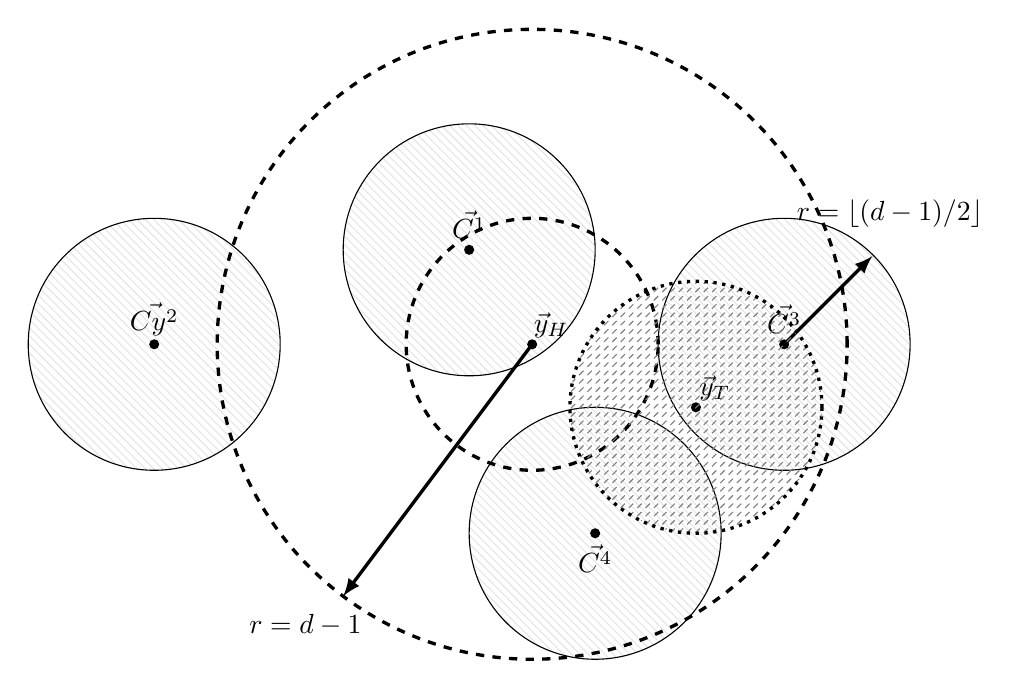
\begin{tikzpicture}[scale=0.80]
      \draw[pattern=north west lines, pattern color=black!10!white] (-6, 0) circle  (2 cm) node at (-6, .4) {$\vec{Cy^2}$};
      \draw[pattern=north west lines, pattern color=black!10!white] (4,0) circle  (2 cm)node at (4,.4) {$\vec{C^3}$};
      \draw[pattern=north west lines, pattern color=black!10!white] (-1,1.5) circle  (2 cm)node at (-1,1.9) {$\vec{C^1}$};
      \draw[pattern=north west lines, pattern color=black!10!white] (1, -3) circle  (2 cm)node at (1, -3.4) {$\vec{C^4}$};
      \draw[fill = black](-6, 0) circle  (2 pt);
      \draw[fill = black](4,0) circle  (2 pt)   ;
      \draw[fill = black](-1,1.5) circle  (2 pt);
      \draw[fill = black] (1, -3) circle  (2 pt) ;
      \draw[fill = black] (0, 0) circle  (2 pt) ;
      \node at (.3,.3) {$\vec{y}_H$};
      \draw [dashed, very thick] (0,0) circle  (2 cm) ;
      \draw [dashed, very thick] (0,0) circle  (5 cm) ;
      \draw [black, very thick, >=latex] [->] (0,0) -- (-3,-4) node[above, pos=1.2] { $r = d-1$};
      \draw [black, very thick, >=latex] [->] (4,0) -- (5.4,1.4) node[above, pos=1.2] { $r = \floor{(d-1)/2}$};
      \draw[fill = black] (2.6,-1) circle  (2 pt) ;
      \node at (2.9,-.7) {$\vec{y}_T$};
      \draw [dotted, very thick, pattern=north east lines, pattern color=gray] (2.6,-1) circle  (2 cm) ;
    \end{tikzpicture}
  }
%  \caption{Decoding using measured soft information and hard decoder } \label{fig:softdecodingML}
\end{figure}




%---------------------------------------------------- fig 4.1

\begin{figure}[!htp]
  \centering
  %\resizebox{0.9\hsize}{!}{
  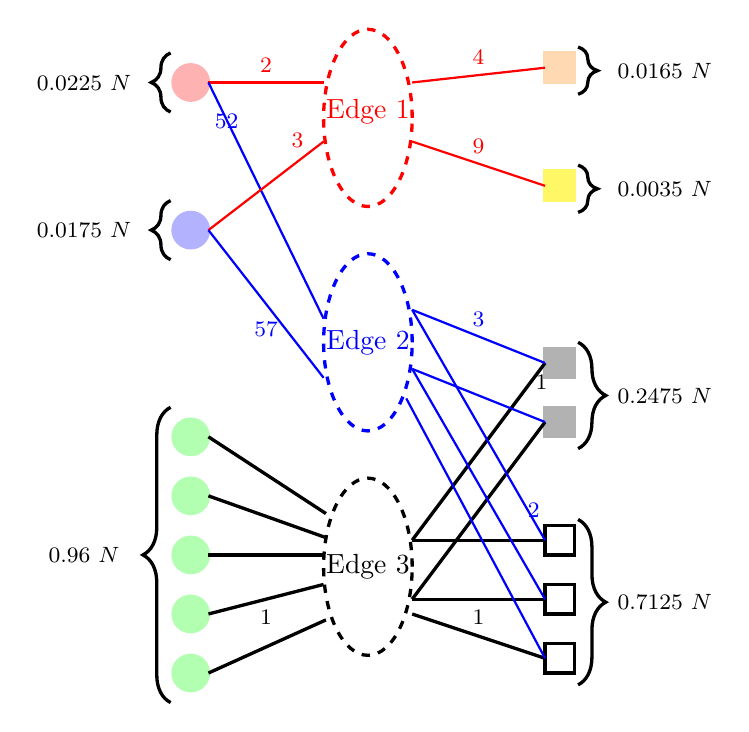
\begin{tikzpicture}[scale=0.75]
    \def \Vn {3}
    \def \Cn {2}
    \def \Ne {3}
    \def \radius {0.3cm}
    \def \vertspace {3.8}
    
    \node at (0, 9.5) [red] {Edge 1};
    \draw [dashed, very thick, red] (0,9.4) ellipse (0.75cm and 1.5cm) ;
    
    \node at (0, 5.6) [blue] {Edge 2};
    \draw [dashed, very thick, blue] (0,5.6) ellipse (0.75cm and 1.5cm) ;
    
    \node at (0, 1.8) [black] {Edge 3};
    \draw [dashed, very thick, black] (0,1.8) ellipse (0.75cm and 1.5cm) ;
    
    \draw [very thick, decorate,decoration={brace,amplitude=7pt},xshift=-4pt,yshift=0pt] (-3.2,9.5) -- (-3.2,10.5) node [black,midway,xshift=-1.1cm]  {\footnotesize $0.0225~N$};
    %\draw [very thick, fill = red!30](-3,11) circle (\radius);
    \draw [red!30, very thick, fill = red!30](-3,10) circle (\radius);
    
    \draw [very thick,decorate,decoration={brace,amplitude=7pt},xshift=-4pt,yshift=0pt] (-3.2,7) -- (-3.2,8) node [black,midway,xshift=-1.1cm] {\footnotesize $0.0175~N$};
    \draw [blue!30, very thick, fill = blue!30](-3,7.5) circle (\radius);
    %\draw [very thick, fill = blue!30](-3,6.5) circle (\radius);
    
    \draw [very thick,decorate,decoration={brace,amplitude=10pt},xshift=-4pt,yshift=0pt] (-3.2,-0.5) -- (-3.2,4.5) node [black,midway,xshift=-1.1cm] {\footnotesize $0.96~N$};
    \draw [green!30, very thick, fill = green!30](-3,2) circle (\radius);
    \draw [green!30, very thick, fill = green!30](-3,1) circle (\radius);
    \draw [green!30, very thick, fill = green!30](-3,0) circle (\radius);
    \draw [green!30, very thick, fill = green!30](-3,4) circle (\radius);
    \draw [green!30, very thick, fill = green!30](-3,3) circle (\radius);
    
    % check-nodes
    \draw [very thick,decorate,decoration={brace, mirror, amplitude=7pt},xshift=-4pt,yshift=0pt] (3.7,9.8) -- (3.7,10.6) node [black,midway,xshift=1.1cm]  {\footnotesize $0.0165~N$};
    \draw [orange!30, very thick, fill = orange!30](3,10) rectangle (3.5,10.5);
    %\draw [very thick, fill = orange!30](3,10) rectangle (3.5,10.5);
    
    
    \draw [very thick,decorate,decoration={brace, mirror, amplitude=7pt},xshift=-4pt,yshift=0pt] (3.7,7.8) -- (3.7,8.6) node [black,midway,xshift=1.1cm] {\footnotesize $0.0035~N$};
    %\draw [very thick, fill = yellow!60] (3,8) rectangle (3.5,8.5);
    \draw [yellow!60, very thick, fill = yellow!60] (3,8) rectangle (3.5,8.5);
    
    \draw [very thick,decorate,decoration={brace, mirror, amplitude=10pt},xshift=-4pt,yshift=0pt] (3.7,3.8) -- (3.7,5.6) node [black,midway,xshift=1.1cm] {\footnotesize $0.2475~N$};
    \draw [black!30, very thick, fill = black!30](3,5) rectangle (3.5,5.5);
    \draw [black!30, very thick, fill = black!30](3,4) rectangle (3.5,4.5);
    
    
    \draw [very thick, decorate,decoration={brace, mirror, amplitude=10pt},xshift=-4pt,yshift=0pt] (3.7,-0.2) -- (3.7,2.6) node [black,midway,xshift=1.1cm] {\footnotesize $0.7125~N$};
    \draw [very thick](3,2) rectangle (3.5,2.5);
    \draw [very thick](3,1) rectangle (3.5,1.5);
    \draw [very thick](3,0) rectangle (3.5,0.5);
    
    %% Edges
    % from Vnode 28 to Edge 1
    \draw[solid,  thick,red] (-2.7,10) -- (-0.75, 10) node [red,above, midway,xshift=-0.0cm,yshift=0.0cm] {\footnotesize $2$};
    %\draw[solid,  thick,red] (-2.7,10) -- (-0.75, 9);% node [red,midway,xshift=-0.6cm,yshift=0.6cm] {\footnotesize $3$};
    
    % from Vnode 28 to Edge 2
    %\draw[solid,  thick,blue] (-2.7,11) -- (-0.75, 6); % node [blue,midway,xshift=-0.5cm,yshift=1.3cm] {\footnotesize $57$};
    \draw[solid,  thick,blue] (-2.7,10) -- (-0.75, 6) node [blue,midway,xshift=-0.5cm,yshift=1.cm] {\footnotesize $52$};
    
    % from Cnode 17 to Edge 1
    \draw[solid,  thick,red] (0.75,10) -- (3, 10.25) node [red,above, midway,xshift=0.0cm,yshift=0.0cm] {\footnotesize $4$};
    %\draw[solid,  thick,red] (0.75,9) -- (3, 10.25);% node [black,midway,xshift=0.6cm,yshift=0.6cm] {\footnotesize $3$};
    
    % from Cnode 15 to Edge 1
    \draw[solid,  thick, red] (0.75,9) -- (3, 8.25) node [red,midway, above, xshift=0.0cm,yshift=-0.0cm] {\footnotesize $9$};
    %\draw[solid,  thick, red] (0.75,10) -- (3, 8.25); % node [black,midway,xshift=0.6cm,yshift=-0.6cm] {\footnotesize $15$};
    
    % from Vnode 36 to Edge 1
    %\draw[solid,  thick,red] (-2.7,7.5) -- (-0.75, 10) ; % node [black,midway,xshift=0.6cm,yshift=0.7cm] {\footnotesize $2$};
    \draw[solid,  thick, red] (-2.7,7.5) -- (-0.75, 9) node [red, below, midway,xshift=0.4cm,yshift=0.8cm] {\footnotesize $3$};
    
    % from Vnode 36 to Edge 2
    %\draw[solid, thick, blue] (-2.7,7.5) -- (-0.75, 6); % node [black,midway,xshift=0.0cm,yshift=0.0cm] {\footnotesize $57$};
    \draw[solid,  thick, blue] (-2.7,7.5) -- (-0.75, 5) node [blue, , below, midway,xshift=0.0cm,yshift=-0.1cm] {\footnotesize $57$};
    
    % from Vnode 1536 to Edge 3
    \draw[solid, very thick, black] (-2.7,1) -- (-0.75, 1.5) node [black,midway, below] {\footnotesize $1$};
    \draw[solid, very thick, black] (-2.7,2) -- (-0.74, 2);
    \draw[solid, very thick, black] (-2.7,0) -- (-0.71, 0.9);
    \draw[solid, very thick, black] (-2.7,3) -- (-0.73, 2.3);
    \draw[solid, very thick, black] (-2.7,4) -- (-0.71, 2.7);
    % node [black,midway,below] {\footnotesize $1$};
    
    % from Cnode 576 to Edge 3
    \draw[solid, very thick, black] (3,4.25) -- (0.75, 1.25); % node [black,midway, below] {\footnotesize $1$};
    \draw[solid, very thick, black] (3,5.25) -- (0.75, 2.25) node [black,midway,above,xshift=0.8cm,yshift=0.65cm] {\footnotesize $1$};
    
    % from Cnode 960 to Edge 3
    \draw[solid, very thick, black] (3,1.25) -- (0.75, 1.25) node [black,midway, below] {\footnotesize $1$};
    \draw[solid, very thick, black] (3,2.25) -- (0.75, 2.25);
    \draw[solid, very thick, black] (3,0.25) -- (0.75, 1.0);% node [black,midway,below] {\footnotesize $1$};
    
    
    % from Cnode 960 to Edge 2
    \draw[solid,thick, blue] (3,4.25) -- (0.75, 5.15); % node [black,midway, above] {\footnotesize $2$};
    \draw[solid,thick, blue] (3,5.25) -- (0.75, 6.15) node [blue,midway,above] {\footnotesize $3$};
    
    % from Cnode 576 to Edge 2
    \draw[solid,thick, blue] (3,1.25) -- (0.75, 5.15); % node [blue,midway,xshift=0.7cm,yshift=-1.3cm] {\footnotesize $3$};
    \draw[solid,thick, blue] (3,2.25) -- (0.75, 6.15) node [blue,midway, above, xshift=0.7cm,yshift=-1.3cm] {\footnotesize $2$};
    \draw[solid,thick, blue] (3,0.25) -- (0.65, 4.65);
  \end{tikzpicture}
  %		}
  %% \caption{Graphical representation of a three-edge type-LDPC code
  %%   presented in \cref{table:rate002designed}, where $\bigcirc$ represents the variable-nodes and $\square$ represents the check-nodes. In addition different node types are demonstrated by different colors. The percentage of node types are shown as fractions of the code length $N$, where $N$ is the number of transmitted code-word bits. This code consists of $3$ different types of variable nodes and $4$ types of check nodes. Also $3$ different edge-types exists}\label{fig:rate002ensemble}
\end{figure}





%----------------------------- shcematic optimization connector


\begin{figure}[!ht]
	\begin{center}
		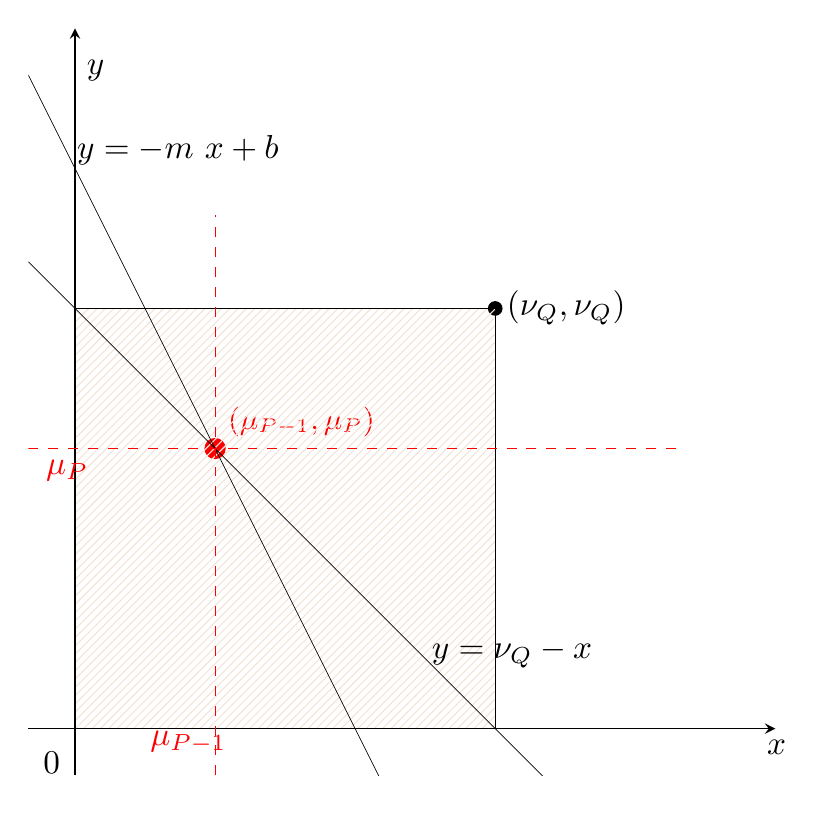
\begin{tikzpicture}[scale=1.2]
		\begin{axis}[
		unit vector ratio*=1 1 1,
		width=11cm,
		grid=major,
		grid style={dashed, green!30},
		axis lines=middle, enlargelimits=false,
		inner axis line style={-stealth},
% 		xlabel={ \textbf{\large $x$} },
% 		xlabel style={
% 			anchor=north west,
% 			align=right
% 		},
% 		ylabel={\textbf{\large $y$}},
% 		ylabel style={
% 			anchor=south east,
% 			align=right
% 		},
		ytick={0},
		xtick={0},
		x tick label style={below , xshift=0.05cm},
		y tick label style={left},
		ymin=-.1,
		ymax=1.5,
		xmin=-0.1,
		xmax=1.5,
		after end axis/.code={
			\path (axis cs:0,0) 
			node [anchor=north west,xshift=7.2cm, yshift=-0.0cm] {$x$}
			node [anchor=north west,xshift=0cm, yshift=7.2cm] {$y$}
			node [anchor=south east,xshift=-0.035cm, yshift=-0.6cm] {0};
		}
		]
		\addplot[fill = red, solid, red](0.3, 0.6) circle  (3 pt) node[below, pos=1.4, xshift = 26pt,yshift = 16pt] { \small $(\mu_{P-1}, \mu_P)$};
		
		\addplot[fill = black, solid, black](.9, .9) circle  (2 pt); % node[below, pos=1.2, xshift = 20pt,yshift = 8pt] { \small $\mu_{P-1}$};
		
		\addplot[solid, very thin, pattern=north east lines, pattern color=brown!20] (0,0) rectangle +(4.45 cm, 4.45 cm) node[right, pos=1, xshift = 0cm, yshift = -0.cm]  {$(\nu_Q, \nu_Q)$};

		\addplot[color=black,very thin] coordinates { (-0.1, 1.0) (1.1, -0.2) } node[right, pos=.7] {$y = \nu_Q-x$};%{ $ m = \dfrac{d_{1,1}^{c}-d_{1,2}^{c}}{d_{1,1}^{v}-d_{1,2}^{v}}$};
		\addplot[color=black,very thin] coordinates { (-0.1,1.4) (0.7, -0.2) } node[right, pos=.1] {$y = -m~x+b$};
		\addplot[color=red,very thin, dashed] coordinates { (0.3,-0.1) (0.3, 1.1) } node[below, pos=.10, xshift = -8pt] { $\mu_{P-1}$};
                \addplot[color=red,very thin, dashed] coordinates { (-0.1,0.6) (1.3, 0.6) } node[below, pos=.10, xshift = -8pt] { $\mu_{P}$};
		\end{axis}
		\end{tikzpicture}
	\end{center}
	%\caption{The schematic representation for one of the connector parts. The itter optimization problem finds set of points like $(\nu_Q, \mu_P)$ and $(\nu_Q, \mu_{P-1})$ on each line where $\mu_P+\mu_{P-1} = \nu_Q$ }\label{fig:answerLinear}
\end{figure}

%------------------------------------- Homodyne

\begin{figure}[!ht]
	\begin{center}
	  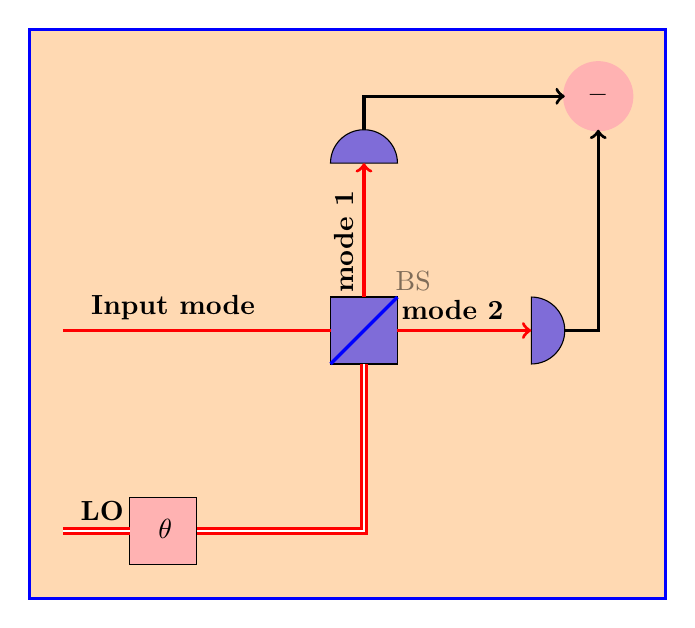
\begin{tikzpicture}[scale=0.85]
            \def \radius {0.5cm}
            
            \draw [blue, very thick, fill=orange!30] (-5.5, 2.5) rectangle (4,11.0);
            \filldraw[fill opacity=0.5,fill=blue] (0cm,9cm) arc (0:180:\radius) -- cycle;
            
            \filldraw[fill opacity=0.5,fill=blue] (2cm, 7cm) arc (90:-90:\radius) -- cycle;
            
            \filldraw [fill  opacity=0.5, fill=blue] (-2*\radius, 6) rectangle (0,7) node [black, xshift = 0.2cm, yshift = 0.2cm] {BS};
            \draw[solid, very thick, blue] (-1,6.) -- (0, 7);
            
             \draw [fill=red!30] (-8*\radius, 3) rectangle (-3,4)  node [black, xshift = -0.4cm, yshift = -0.4cm] {$\theta$};
            
            \draw [red!30, very thick, fill = red!30](3,10) circle (\radius) node [black] {\textbf{--}};
            
            \draw[solid, very thick, red] (-5,6.5) -- (-1, 6.5) node[black, xshift = -2cm, above] {\textbf{Input mode}};
            \draw[solid, very thick, red, double] (-5,3.5) node[black, xshift = 0.5cm, above] {\textbf{LO}} -- (-4, 3.5) (-3, 3.5) -- (-0.5, 3.5) -- (-0.5, 6) ;
            
            \draw[solid, very thick, red, ->] (0,6.5) -- (2, 6.5) node[black, xshift = -1cm, above] {\textbf{mode 2}};
            \draw[solid, very thick, red, ->] (-0.5,7) -- (-0.5, 9) node[black, yshift = -1cm, above, rotate = 90] {\textbf{mode 1}};
            
            
            \draw[solid, very thick, black, ->] (2.5,6.5) -- (3, 6.5) -- (3, 9.5);
            \draw[solid, very thick, black, ->] (-0.5,9.5) -- (-0.5, 10) -- (2.5, 10);
		\end{tikzpicture}
	\end{center}
	%\caption{The schematic representation for one of the connector parts. The itter optimization problem finds set of points like $(\nu_Q, \mu_P)$ and $(\nu_Q, \mu_{P-1})$ on each line where $\mu_P+\mu_{P-1} = \nu_Q$ }\label{fig:answerLinear}
\end{figure}




%------------------------------- MLC-MSD forward
\begin{figure*}[!ht]
	\centering
% 		{%\resizebox{14cm}{9 cm}
		\resizebox{0.8\textwidth}{!}{
			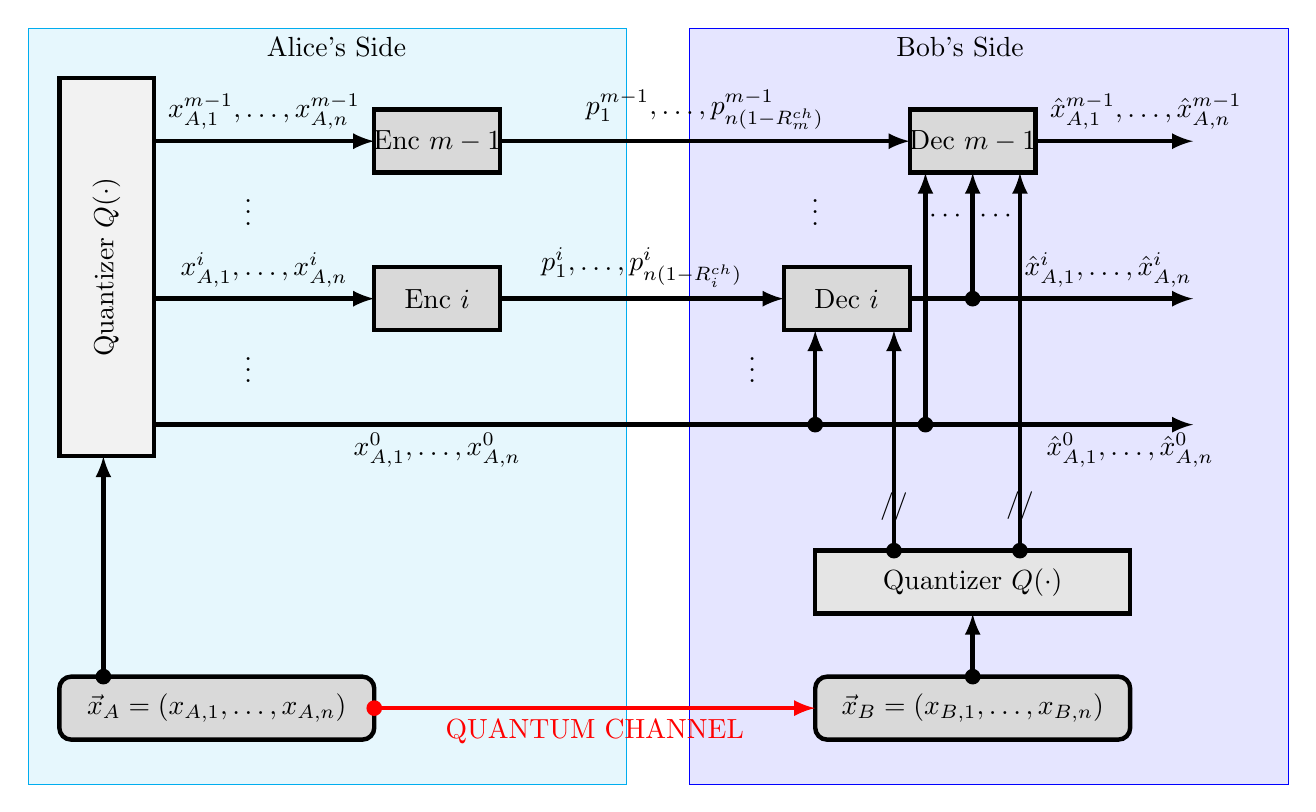
\begin{tikzpicture}[scale=0.8, 
			dot/.style    = {anchor=base,fill,circle,inner sep=2pt},
			block_1/.style  = {draw, rectangle, black, ultra thick, fill=gray!30!white, minimum width = 0.75cm, minimum height = 0.75cm},]
			
			
			\draw[cyan, ultra thin, fill=cyan!10!white] (0.0,-8.2) rectangle ++(9.5,12) node at (4.9,3.5) [black]{Alice's Side};
			\draw[blue, ultra thin, fill=blue!10!white] (10.5,-8.2) rectangle ++(9.5,12)  node at (14.8,3.5) [black]{Bob's Side};
			
			%% QUANTUM CHANNEL AT THE BOTOM
			\draw[black, ultra thick, fill=gray!30!white, rounded corners=1ex] (0.5,-7.5) rectangle ++(5,1) node[pos=.5] {$\vec{x}_A = (x_{A,1}, \dots, x_{A,n})$};
			\draw[black, ultra thick, fill=gray!30!white, rounded corners=1ex] (12.5,-7.5) rectangle ++(5,1) node[pos=.5] {$\vec{x}_B = (x_{B,1}, \dots, x_{B,n})$};
			\draw[black, ultra thick, fill=black!10!white] (12.5,-5.50) rectangle ++(5,1) node[pos=.5] {Quantizer $Q(\cdot)$};
			\draw [black, ultra thick, >=latex] [->] (15,-6.5) coordinate[dot] -- (15,-5.5) ;
			\draw [red, ultra thick, >=latex] [->] (5.5,-7) coordinate[dot] -- (12.5,-7) node[pos=0.5, below]{QUANTUM CHANNEL};
			
			
			% CLASSICAL CHANNEL
			\draw[black, ultra thick, fill=gray!10!white] (.5,-3) rectangle ++(1.5,6) node[rotate=90,pos=0.5]{Quantizer $Q(\cdot)$};
			\draw [black, ultra thick, >=latex] [->] (1.2,-6.5) coordinate[dot] -- (1.2,-3) ;
			% ENCODER SIDE:
			\draw [black, ultra thick, >=latex] [->] (2,2) -- (5.5,2) node[above, pos=.5] { $x_{A,1}^{m-1},\ldots, x_{A,n}^{m-1}$};
			\draw [black, ultra thick, >=latex] [->] (2,-.5) -- (5.5,-.5) node[above, pos=.5] { $x_{A,1}^i,\ldots, x_{A,n}^i$};
			\draw [black, ultra thick, >=latex] [->] (2,-2.5) -- (18.5,-2.5);
			\draw[black, ultra thick, fill=gray!30!white] (5.5,1.5) rectangle ++(2,1) node[pos=.5] {Enc $m-1$};
			\draw[black, ultra thick, fill=gray!30!white] (5.5,-1) rectangle ++(2,1) node[pos=.5] {Enc $i$};
			\draw [black, ultra thick, >=latex] [->] (7.5,2) -- (14,2) node[above, pos=.5] { $p_1^{m-1},\ldots, p_{n(1-R^{ch}_m)}^{m-1}$};
			\draw [black, ultra thick, >=latex] [->] (7.5,-.5) -- (12,-.5) node[above, pos=.5] { $p_1^i,\ldots, p_{n(1-R^{ch}_i)}^i$};
			%% DECODER SIDE
			\draw[black, ultra thick, fill=gray!30!white] (12,-1) rectangle ++(2,1) node[pos=.5] {Dec $i$};
			\draw[black, ultra thick, fill=gray!30!white] (14,1.5) rectangle ++(2,1) node[pos=.5] {Dec $m-1$};
			\draw [black, ultra thick, >=latex] [->] (16,2) -- (18.5,2) node [pos = 0.7, above] {$\hat{x}_{A,1}^{m-1},\ldots, \hat{x}_{A,n}^{m-1}$};
			\draw [black, ultra thick, >=latex] [->] (14,-.5) -- (18.5,-.5) node [pos=.7, above] {$\hat{x}_{A,1}^i,\ldots, \hat{x}_{A,n}^i$};
			%% VERTICAL LINES AND DOTS
			\draw [black, ultra thick, >=latex] [->] (12.5,-2.5) coordinate[dot] -- (12.5,-1) ;
			\draw [black, ultra thick,  >=latex] [->] (13.75,-4.5) coordinate[dot] -- (13.75,-1) node [pos=.2]{//};
			\draw [black, ultra thick, >=latex] [->] (14.25,-2.5) coordinate[dot] -- (14.25,1.5) ;
			\draw [black, ultra thick, >=latex] [->] (15,-.5) coordinate[dot] -- (15,1.5) ;
			\draw [black, ultra thick, >=latex] [->] (15.75,-4.5) coordinate[dot] -- (15.75,1.5) node [pos=.12]{//};
			\node at (17.5,-2.9) {$\hat{x}_{A,1}^0,\ldots, \hat{x}_{A,n}^0$};
			\node at (6.5,-2.9) {$x_{A,1}^0,\ldots, x_{A,n}^0$};
			\node at (3.5,-1.5) {$\vdots$};
			\node at (11.5,-1.5) {$\vdots$};
			\node at (3.5,1.) {$\vdots$};
			\node at (12.5,1.) {$\vdots$};
			\node at (14.6,0.8) {$\cdots$};
			\node at (15.4,0.8) {$\cdots$};
% 			\node at (17.5,.4) {$\hat{x}_{B,1}^i,\ldots, \hat{x}_{B,n}^i$};
% 			\node at (13.8,-3.8) {$\vecXA = (x_{A,1},\,\,\, \ldots,\, x_{A,n})$};
% 	\node at (17.5,2.4) {$\hat{x}_{B,1}^{m-1},\ldots, \hat{x}_{B,n}^{m-1}$};
			\end{tikzpicture}
		}
	%% \caption{The MLC-MSD scenario for the reverse reconciliation. First the input source is quantized into an $m$-bit source. Then each of the $m$ sources is encoded and sent to Alice. The decoder has the side information from its own source and with the $m$ encoded sources produces an estimate of the quantized source. Usually we transmit the least significant bits directly to the channel.}\label{fig:ChannelCodingRR}
\end{figure*}




%------------------------------- Shortening 
\begin{figure*}[!ht]
  \centering
  % 		{%\resizebox{14cm}{9 cm}
  \resizebox{0.8\textwidth}{!}{
    \begin{tikzpicture}[scale=0.8, 
	dot/.style    = {anchor=base,fill,circle,inner sep=2pt},
	block_1/.style  = {draw, rectangle, black, ultra thick, fill=gray!30!white, minimum width = 0.75cm, minimum height = 0.75cm},]


       \draw [black, ultra thick, >=latex] [->] (-1,0) -- (1,0) node[above, pos=.5] {$k-s$};
       \draw[black, ultra thick, fill=blue!10!white, rounded corners=1ex] (1,-1.) rectangle ++(3,2) node[pos=.5, yshift=0.5cm] {\textbf{Insert}};
       \node at (2.5,-0.5) {\footnotesize{$s$ known symbols}};
       
       \draw [black, ultra thick, >=latex] [->] (4,0) -- (5,0) node[above, pos=.5] {$k$};
       \draw[black, ultra thick, fill=gray!30!white, rounded corners=1ex] (5,-1.) rectangle ++(3,2) node[pos=.5, yshift = 0.5cm] {\textbf{Encoder} };
       \node at (6.5,-0.5) {\footnotesize{$R = \dfrac{k/n}$}};

       \draw [black, ultra thick, >=latex] [->] (8,0) -- (9,0) node[above, pos=.5] {$n$};
       \draw[black, ultra thick, fill=red!30!white, rounded corners=1ex] (9,-1.) rectangle ++(3,2) node[pos=.5, yshift = 0.5cm] {\textbf{Discard} };
       \node at (10.5,-0.5) {\footnotesize{$s$ known symbols}};

       \draw [black, ultra thick, >=latex] [->] (12,0) -- (14,0) node[above, pos=.5] {$n-s$};
      


       
       


       \draw [black, ultra thick, >=latex] [<-] (-1,0-5) -- (1,0-5) node[above, pos=.5] {$k-s$};
       \draw[black, ultra thick, fill=red!30!white, rounded corners=1ex] (1,-1.-5) rectangle ++(3,2) node[pos=.5, yshift=0.5cm] {\textbf{discard}};
       \node at (2.5,-0.5-5) {\footnotesize{$s$ known symbols}};
       
       \draw [black, ultra thick, >=latex] [<-] (4,0-5) -- (5,0-5) node[above, pos=.5] {$k$};
       \draw[black, ultra thick, fill=gray!30!white, rounded corners=1ex] (5,-1.-5) rectangle ++(3,2) node[pos=.5, yshift = 0.5cm] {\textbf{Decoder} };
       \node at (6.5,-0.5-5) {\footnotesize{$R = \dfrac{k/n}$}};

       \draw [black, ultra thick, >=latex] [<-] (8,0-5) -- (9,0-5) node[above, pos=.5] {$n$};
       \draw[black, ultra thick, fill=blue!10!white, rounded corners=1ex] (9,-1.-5) rectangle ++(3,2) node[pos=.5, yshift = 0.5cm] {\textbf{Insert} };
       \node at (10.5,-0.5-5) {\footnotesize{$s$ known symbols}};

       \draw [black, ultra thick, >=latex] [<-] (12,0-5) -- (14,0-5) node[above, pos=.5] {$n-s$};

       
    \end{tikzpicture}
  }
\end{figure*}




%%%%%%%%%%%%%%%%%%%%%%%%%%%% rate reagion


\begin{figure}[!ht]
	\begin{center}
		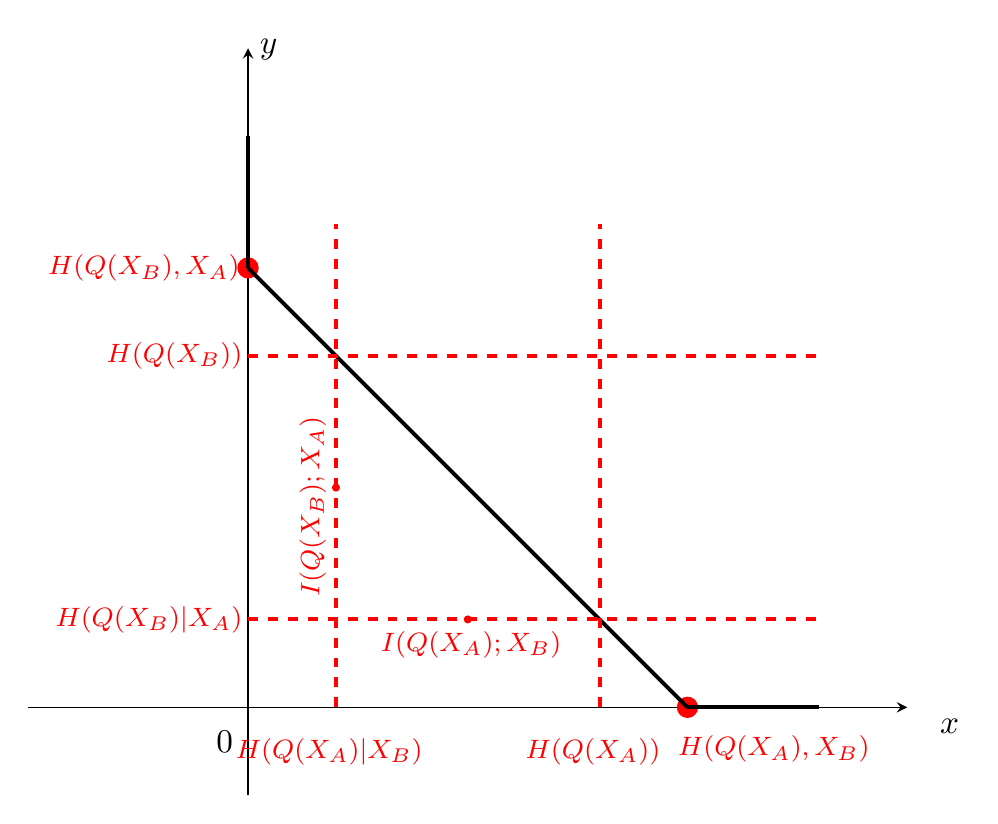
\begin{tikzpicture}[scale=1.2]
		\begin{axis}[
		unit vector ratio*=1 1 1,
		width=11cm,
		grid=major,
		grid style={dashed, green!30},
		axis lines=middle, enlargelimits=false,
		inner axis line style={-stealth},
		ytick={0},
		xtick={0},
		x tick label style={below , xshift=0.05cm},
		y tick label style={left},
		ymin=-.2,
		ymax=1.5,
		xmin=-0.5,
		xmax=1.5,
		after end axis/.code={
			\path (axis cs:0,0) 
			node [anchor=north west,xshift=7.2cm, yshift=-0.0cm] {$x$}
			node [anchor=north west,xshift=0cm, yshift=7.2cm] {$y$}
			node [anchor=south east,xshift=-0.035cm, yshift=-0.6cm] {0};
		}
		]

                  \addplot[fill = red, solid, red](1.0, 0.0) circle  (3 pt) node[below, pos=1.4, xshift = 26pt,yshift = -5pt]{ \footnotesize{$H(Q(X_A),X_B)$}};

                  \addplot[fill = red, solid, red](0.0, 1.0) circle  (3 pt) node[left, pos=0.1, xshift = 1pt,yshift = -0pt]{ \footnotesize{$H(Q(X_B),X_A)$}};

                  \addplot[fill = red, solid, red](0.5, 0.2) circle  (1 pt) node[below, pos=0.1, xshift = 1pt,yshift = -0pt]{ \footnotesize{$I(Q(X_A);X_B)$}};
                   \addplot[fill = red, solid, red](0.2, 0.5) circle  (1 pt) node[left, pos=0.5, xshift = -7pt,yshift = 25pt, rotate=90]{ \footnotesize{$I(Q(X_B);X_A)$}};
		
		
%%		\addplot[solid, very thin, pattern=north east lines, pattern color=brown!20] (0,0) rectangle +(4.45 cm, 4.45 cm) node[right, pos=1, xshift = 0cm, yshift = -0.cm]  {$(\nu_Q, \nu_Q)$};

		  \addplot[color=black,very thick] coordinates { (-0.0, 1.0) (1.0, -0.0) };
                  \addplot[color=black,very thick] coordinates { (-0.0, 1.0) (0.0, 1.3) };
                  \addplot[color=black,very thick] coordinates { (1.0, 0.0) (1.3, 0.0) };
                  
		  \addplot[color=red,very thick, dashed] coordinates { (0.8,-0.0) (0.8, 1.1) } node[below, pos=.10, xshift = -2pt, yshift = -20pt] { \footnotesize{$H(Q(X_A))$}};
                  \addplot[color=red,very thick, dashed] coordinates { (0.2,-0.0) (0.2, 1.1) } node[below, pos=.10, xshift = -2pt, yshift = -20pt] { \footnotesize{$H(Q(X_A)|X_B)$}};
                  
                  \addplot[color=red,very thick, dashed] coordinates { (-0.0,0.8) (1.3, 0.8) } node[left, pos=.10, xshift = -15pt, yshift = 0pt] { \footnotesize{$H(Q(X_B))$}};
                  \addplot[color=red,very thick, dashed] coordinates { (-0.0,0.2) (1.3, 0.2) } node[left, pos=.10, xshift = -15pt, yshift = 0pt] { \footnotesize{$H(Q(X_B)|X_A)$}};
		\end{axis}
		\end{tikzpicture}
	\end{center}
	%\caption{The schematic representation for one of the connector parts. The itter optimization problem finds set of points like $(\nu_Q, \mu_P)$ and $(\nu_Q, \mu_{P-1})$ on each line where $\mu_P+\mu_{P-1} = \nu_Q$ }\label{fig:answerLinear}
\end{figure}




%======================================= chennels BIOSM
\begin{figure}[!htbp]
  \centering
  \resizebox{.8\hsize}{!}{
    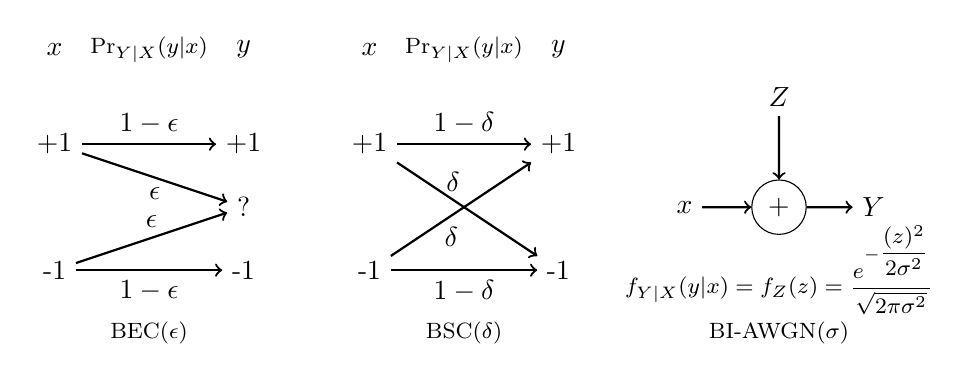
\begin{tikzpicture}[scale=0.8]
      \def\c0{0}% scalebar-x at golden ratio of x=1728px
      \def\c1{-2}
      \def\goup{2}
      \def\gort{3}
      \def\bscx{5}
      \def\awgn{10}
      % -------------------------------------------- BEC(e)
      % set the nodes
      \node at (0, 0)   (bec_in_0) {+1};
      \node at (0,0-\goup)   (bec_in_1) {-1};
      \node at (\gort, 0)   (bec_out_0) {+1};
      \node at (\gort,0-\goup)   (bec_out_1) {-1};
      \node at (\gort,1-\goup)   (bec_out_2) {?};
      % draw edges
      \draw[solid, thick, ->] (bec_in_0) -- (bec_out_0) node [midway, above] {$1-\epsilon$};
      \draw[solid, thick, ->] (bec_in_1) -- (bec_out_1) node [midway, below] {$1-\epsilon$};
      \draw[solid, thick, ->] (bec_in_0) -- (bec_out_2) node [midway, below] {$\epsilon$};
      \draw[solid, thick, ->] (bec_in_1) -- (bec_out_2) node [midway, above] {$\epsilon$};
      % -------------------------------------------- BSC(delta)
      % set the nodes
      \node at (\bscx, 0)   (bsc_in_0) {+1};
      \node at (\bscx,-2)   (bsc_in_1) {-1};
      \node at (\bscx+\gort, 0)   (bsc_out_0) {+1};
      \node at (\bscx+\gort,-2)   (bsc_out_1) {-1};
      % draw edges
      \draw[solid, thick, ->] (bsc_in_0) -- (bsc_out_0) node [midway, above] {$1-\delta$};
      \draw[solid, thick, ->] (bsc_in_1) -- (bsc_out_1) node [midway, below] {$1-\delta$};
      \draw[solid, thick, ->] (bsc_in_0) -- (bsc_out_1) node [midway, below, xshift = -0.2cm, yshift = -0.1cm] {$\delta$};
      \draw[solid, thick, ->] (bsc_in_1) -- (bsc_out_0) node [midway, above, xshift = -0.1cm, yshift = 0.1cm] {$\delta$};
      % -------------------------------------------- AWGN(sigma)
      \node at (\awgn, 1-\goup)   (bawgn_x) {$x$};
      \node at (\awgn+\gort/2, \goup-1.25)   (bawgn_n) {$Z$};
      \node at (\awgn+\gort, 1-\goup)   (bawgn_y) {$Y$};
      \node[draw, circle] at (\awgn+\gort/2,  1-\goup) (adder) {$+$};

      \draw[solid, thick, ->] (bawgn_x) -- (adder);
      \draw[solid, thick, ->] (bawgn_n) -- (adder);
      \draw[solid, thick, ->] (adder) -- (bawgn_y);
      % -------------------------------------------- Names
      \node at (0, \goup-0.5) () {$x$};
      \node at (\gort,\goup-0.5) () {$y$};
      \node at (\gort/2,\goup-0.5) () {\footnotesize{$\Pr_{Y|X}(y|x)$}};
      \node at (\gort/2,1-2*\goup) () {\footnotesize{BEC$(\epsilon)$}};

      \node at (\bscx, \goup-0.5) () {$x$};
      \node at (\bscx+\gort,\goup-0.5) () {$y$};
      \node at (\bscx+\gort/2,\goup-0.5) () {\footnotesize{$\Pr_{Y|X}(y|x)$}};
      \node at (\bscx+\gort/2,1-2*\goup) () {\footnotesize{BSC$(\delta)$}};

      \node at (\awgn+\gort/2,0-\goup) () {\footnotesize{$f_{Y|X}(y|x) = f_Z(z) = \dfrac{e^{-\dfrac{(z)^2}{2\sigma^2}}}{\sqrt{2\pi\sigma^2}}$}};
      \node at (\awgn+\gort/2,1-2*\goup) () {\footnotesize{BI-AWGN$(\sigma)$}};
    \end{tikzpicture}
  }
%  \caption{The schematic representation of standard BIOSM channels}\label{fig:biosm}
\end{figure}










\pgfmathdeclarefunction{gauss}{2}{\pgfmathparse{1/(#2*sqrt(2*pi))*exp(-((x-#1)^2)/(2*#2^2))}%
}
\begin{figure}[h]
    \centering
    \resizebox{1.0\hsize}{!}{
    \begin{tikzpicture}
\begin{axis}[no markers, domain=-9:8, samples=100,
axis lines =left, 
%axis lines*= middle,
% xlabel=Test, 
ylabel= probability,
height=6cm, width=21cm,
xticklabels={-9, -8, ...,7, 8}, ytick=\empty, enlargelimits=false, clip=false, axis on top, grid = major]
\addplot [fill=gray!20, draw=none, domain=-8:9] {gauss(0,2)} \closedcycle;
\addplot [fill=red!70, draw=none, domain=2:3] {gauss(0,2)} \closedcycle;
\addplot [fill=red!70, draw=none, domain=-6:-5] {gauss(0,2)} \closedcycle;
\end{axis}
\node[gray, text width=1cm] at (1,-1.5) {0\\0\\0\\0};
\node[gray, text width=1cm] at (2.1,-1.5) {0\\0\\0\\1};
\node[text width=1cm] at (3.2,-1.5) {\textbf{0}\\\color{red}{\textbf{0}}\\\textbf{1}\\\textbf{0}\color{black}};
\node[gray, text width=1cm] at (4.3,-1.5) {0\\0\\1\\1};
\node[gray, text width=1cm] at (5.4,-1.5) {0\\1\\0\\0};
\node[gray, text width=1cm] at (6.6,-1.5) {0\\1\\0\\1};
\node[gray, text width=1cm] at (7.8,-1.5) {0\\1\\1\\0};
\node[gray, text width=1cm] at (9,-1.5) {0\\1\\1\\1};
\node[gray, text width=1cm] at (10.1,-1.5) {1\\0\\0\\0};
\node[gray, text width=1cm] at (11.3,-1.5) {1\\0\\0\\1};
\node[text width=1cm] at (12.45,-1.5) {\textbf{1}\\\color{red}{\textbf{0}}\\\textbf{1}\\\textbf{0}\color{black}};
\node[gray, text width=1cm] at (13.6,-1.5) {1\\0\\1\\1};
\node[gray, text width=1cm] at (14.8,-1.5) {1\\1\\0\\0};
\node[gray, text width=1cm] at (15.9,-1.5) {1\\1\\0\\1};
\node[gray, text width=1cm] at (17.,-1.5) {1\\1\\1\\0};
\node[gray, text width=1cm] at (18.1,-1.5) {1\\1\\1\\1};
\end{tikzpicture}
}
    \caption{(Color online) The binary outputs of a $4$-level quantizer. The top row denotes the most significant bits and the lowest row represents the least significant bit. Individually each row can be considered as a source with equi-probable binary outputs. But knowing the correct values of low significant bits give information about the most significant bit.}
    \label{fig:my_label}
\end{figure}





%++++++++++++++++++++++++++
%================================= Tanner graph
\begin{figure}[h]
    \centering
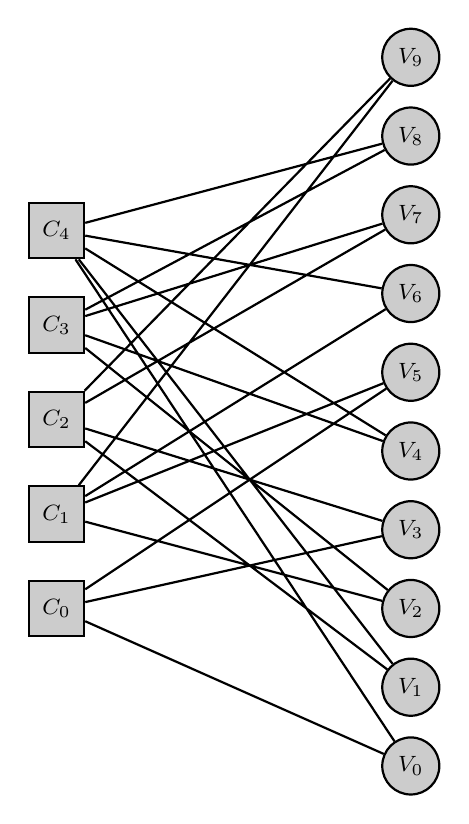
\begin{tikzpicture}
\foreach \i in {0,...,9}
{
        \pgfmathtruncatemacro{\label}{\i};
        \node[circle,thick,draw=black,fill=white!80!black,minimum size=5]
        (v\label) at (0, \i) {\footnotesize{$V_\label$}};
}

\foreach \j in {0,...,4}
{
        \pgfmathtruncatemacro{\label}{\j};
        \node  (c\label) at (-4.5, 1.2*\j+2) [draw,thick,fill=white!80!black,minimum width=20,minimum height=20] {\footnotesize{$C_\label$}};
}

% \tikzstyle{every node}=[draw];
\draw[thick] (v0) -- (c0) (v0) -- (c4)
(v1) -- (c2) (v1) -- (c4)
(v2) -- (c1) (v2) -- (c3)
(v3) -- (c0) (v3) -- (c2)
(v4) -- (c3) (v4) -- (c4)
(v5) -- (c0) (v5) -- (c1)
(v6) -- (c1) (v6) -- (c4)
(v7) -- (c2) (v7) -- (c3)
(v8) -- (c3) (v8) -- (c4)
(v9) -- (c1) (v9) -- (c2);
\end{tikzpicture}
\end{figure}


\end{document}
